\documentclass[10pt,a4paper]{article}
\usepackage{amsmath,amssymb,amsthm,graphicx}
\usepackage{amsmath,amssymb,amsthm,hyperref,tikz,enumerate,subfigure}
\newtheorem{theorem}{Theorem}[section]
\newtheorem{theo}[theorem]{Theorem}
\newtheorem{lemm}[theorem]{Lemma}
\newtheorem{prop}[theorem]{Proposition}
\newtheorem{defi}[theorem]{Definition}
\newtheorem{rema}[theorem]{Remark}
\DeclareMathSymbol{\leqslant}{\mathalpha}{AMSa}{"36}
\DeclareMathSymbol{\geqslant}{\mathalpha}{AMSa}{"3E}
\DeclareMathSymbol{\eset}{\mathalpha}{AMSb}{"3F}
\renewcommand{\leq}{\;\leqslant\;}
\renewcommand{\geq}{\;\geqslant\;}
%\newcommand{\dd}{\,\text{\rm d}}




\newcommand{\la}{\label}
\newcommand{\Om}{\Omega}


\newcommand{\e}{\varepsilon}
\newcommand{\h}{\frac{1}{2}}

\newcommand{\rhoN}{\rho^{\pi}}
\newcommand{\si}{\sigma}
\newcommand{\tc}{\, |\, }

\newcommand{\scalar}[2]{\langle #1, #2\rangle}



\DeclareMathOperator*{\union}{\bigcup}
\DeclareMathOperator*{\inter}{\bigcap}
\DeclareMathOperator{\var}{Var}
\newcommand{\tv}{\mathrm{TV}}
\newcommand{\ent}{\mathrm{Ent}}
\newcommand{\gap}{\mathrm{gap}}
\newcommand{\rBe}{\mathrm{Be}}
\newcommand{\IND}{\mathbf{1}}
\newcommand{\ind}{\mathbf{1}}

\newcommand{\cA}{\mathcal{A}}
\newcommand{\cB}{\mathcal{B}}
\newcommand{\cE}{\mathcal{E}}
\newcommand{\cL}{\mathcal{L}}
\newcommand{\cP}{\mathcal{P}}
\newcommand{\cS}{\mathcal{S}}
\newcommand{\cT}{\mathcal{T}}
\newcommand{\cU}{\mathcal{U}}
\newcommand{\cV}{\mathcal{V}}
\newcommand{\bbC}{\mathbb{C}}
\newcommand{\bbE}{\mathbb{E}}

\newcommand{\bbN}{\mathbb{N}}
\newcommand{\bbP}{\mathbb{P}}
\newcommand{\bbR}{\mathbb{R}}
\newcommand{\bbS}{\mathbb{S}}


%\DeclareMathOperator{\cov}{Cov}
%\DeclareMathOperator{\Hess}{Hess}
%\DeclareMathOperator{\dist}{dist}
%\DeclareMathOperator{\osc}{osc}
%\DeclareMathOperator{\Id}{Id}
%\DeclareMathOperator{\diag}{diag}
%\DeclareMathOperator{\supp}{supp}
%\DeclareMathOperator{\PI}{PI}
%\DeclareMathOperator{\Ent}{Ent}




\let\a=\alpha
\let\b=\beta
\let\d=\delta
\let\e=\varepsilon
\let\g=\gamma
\let\l=\lambda
\let\o=\omega
\let\r=\rho
\let\t=\tau
\let\z=\zeta
\let\G=\Gamma
\let\O=\Omega





%%%%%%%%%%%%%%%%%%%%%%%%%%%%%%%%%%%%%%%%%%%%%%%%%%%%%%%%%%%%%%%%%%%%%%%%%%%%%%%%%%%%%%%%%%%%%%%%%%%
\graphicspath{{./figures/}}

\newcommand*{\mk}{\mkern -1mu}
\newcommand*{\Mk}{\mkern -2mu}
\newcommand*{\mK}{\mkern 1mu}
\newcommand*{\MK}{\mkern 2mu}

\hypersetup{urlcolor=purple, linkcolor=blue, citecolor=red}

\newcommand*{\romanenumi}{\renewcommand*{\theenumi}{\roman{enumi}}}
\newcommand*{\Romanenumi}{\renewcommand*{\theenumi}{\Roman{enumi}}}
\newcommand*{\alphenumi}{\renewcommand*{\theenumi}{\alph{enumi}}}
\newcommand*{\Alphenumi}{\renewcommand*{\theenumi}{\Alph{enumi}}}
\let\oldtilde\tilde
\renewcommand*{\tilde}[1]{\mathchoice{\widetilde{#1}}{\widetilde{#1}}{\oldtilde{#1}}{\oldtilde{#1}}}
\let\oldhat\hat
\renewcommand*{\hat}[1]{\mathchoice{\widehat{#1}}{\widehat{#1}}{\oldhat{#1}}{\oldhat{#1}}}
\let\oldforall\forall
\renewcommand*{\forall}{\mathrel{\oldforall}}
\usepackage{cleveref}
\crefname{originalTheorem}{original Theorem}{original Theorems}
\Crefname{originalTheorem}{Original Theorem}{Original Theorems}
\makeatletter
\newlabel{th:unifintime}{{1.5}{source}{}{sourcepointer-1}{}}
\newlabel{th:unifintime@cref}{{[originalTheorem][0][]1.5}{[1][0][]source}{}{}{}}
\makeatother
\title{Uniform-in-time propagation of chaos for finite nonlinear recombinations with explicit empirical initial error}
\author{Pietro Caputo, Daniel Parisi}
\date{doi:10.5802/ahl.219:published-2024; CC BY 4.0}
\begin{document}
\maketitle
\noindent\textit{Editorial note.} The quantitative statement retains the initial empirical Hamming-Wasserstein error. No canonical conditioning rate or unreviewed local central limit theorem is assumed.\par\medskip
\noindent\textit{Editorial note.} The original Section3.4 reuses Q for the full vector field Q(p)-p from the earlier gain-operator convention. Its explicit bilinear formula and displayed vector field1318 determine the meaning.\par\medskip
\noindent\textit{Editorial note.} The variational solution is defined by1323-1330 along q\_t=S\_t(q). The fixed-base ordinary semigroup display1331-1333 is not selected or used. The generator comparison relies instead on the separately proved identity1786-1821. No replacement flow formula is inserted into the author text.\par\medskip
\noindent\textit{Editorial note.} At1370 the initial term for h\_t=bar S\_t(q)(p) is determined by h0=p and the following explicit u/v equations1374. The printed q is an initial-value symbol slip; retain the author display and disclose it.\par\medskip
\noindent\textit{Editorial note.} In1856/1860 the coarse error estimates have factor4. Keeping it through the product expansion gives a valid K\_s no larger than4k e\textasciicircum{}(-Ds)(n\textasciicircum{}5+(k-1)n\textasciicircum{}4 e\textasciicircum{}(-Ds))/N\textasciicircum{}2 for normalized tests. Its integral after multiplyingN/2 is at most2k\textasciicircum{}2n\textasciicircum{}5(1-e\textasciicircum{}(-Dt))/(DN), below the coefficient4 printed in the counted theorem920. The smaller intermediate display1864/1868 is not separately certified.\par\medskip
\noindent\textit{Editorial note.} At1862 the particle pair indices run up to N, as in the generator and1827, not the n sites printed there. Several native displays1511/1780/1801/1832 contain unmatched layout parentheses; any necessary delimiter adaptation must preserve their actual author expressions and be recorded mechanically.\par\medskip
\noindent\textit{Editorial note.} The original source1207-1212 pair-in-V notation means inclusion of both coordinates. Original1172-1179 crosses a left delimiter inside an aligned display; retain mathematics when applying any required layout-only delimiter handling.\par\medskip
\noindent\textit{Editorial note.} Source1674 writes an equality for the expected Wasserstein distance, while the explicitly constructed coupling in1661–1664 only establishes the required upper bound. Equality need not hold because that coupling need not be optimal. The subsequent calculation uses only this upper bound. Preserve the original formula and read this intermediate step as the already-established inequality; no new proof or changed conclusion is supplied.\par\medskip
\noindent\textit{Editorial scope.} One quantitative empirical-initial-error theorem only. The derivative estimate and W monotonicity are uncounted supporting proofs. The canonical O(N\textasciicircum{}-1/2) result305-316 and its local-CLT/equivalence-of-ensembles chain are not claimed prepared by this task.\par\medskip
\noindent\textit{Allowed standard prerequisites (editorial).}\begin{itemize}
\item Finite-dimensional polynomial ODE existence, variation equations and finite continuous-time Markov generators. Only general finite-dimensional calculus. The model-specific derivative contraction, second-order bound and generator cancellation are retained local obligations.
\item Optimal couplings on finite spaces, convexity of Wasserstein distance, product telescoping and Tonelli. Basic tools; the marked-tree cancellation and uniform-in-time bounds are not supplied as free theorems.
\item Sampling with versus without replacement for a symmetric N-particle law. For a bounded k-particle test, replacing sampling of distinct labels by iid labels changes its expectation by at most2*||test||\_infinity times the probability of a repeated label, bounded by k(k-1)/(2N).. Justifies the ordinary T1 sampling term; the author uses the looser2k(k-1)/N.
\end{itemize}\medskip
\ifdefined\hypertarget\hypertarget{sourcepointer-1}{}\fi
\noindent\textit{Source reference.} Original Theorem 1.5: sources/nonlinear-recombinations-ahl-2024-219/source0.tex, source lines 305--316. The source introduction states the eventual application. This task counts the stronger explicit empirical-error estimate916-924 and proves it without the canonical-initial specialization or local-CLT chain.\par\medskip
\paragraph{Scope of the quantitative propagation estimate.}
Fix the finite recombination space with $n\ge2$ sites, a separating measure $\nu$,
and $N$ particles. In the displayed estimate take $1\le k\le N$.
The probability measures $\mu_N$ are symmetric as in the author's definition of chaos.
The empirical law, the Hamming--Wasserstein distance and the particle generator
are those defined in the original source below. The estimate retains its initial
empirical-distance term; it does not assert the separate canonical-initial-data rate.

\subsection{The nonlinear equation}\label{setup}
Let $\Omega = \prod_{i=1}^nX_i$ be the set of $n$-vectors $\sigma = (\sigma_1,\,\dots,\,\sigma_n)$ where $\si_i\in X_i$, and the $X_i$ are given finite sets. We interpret $\si$ as a particle. Thus, a particle is a string of $n$ characters each taken from a finite alphabet. A basic example is obtained by taking $\Omega=\{0,1\}^n$. Without loss of generality we will assume that each $X_i$ has the form $X_i :=\{0,1,2,\,\dots,\,q_i\}$, for some $q_i \in \bbN$. Given a subset $A \subset [n],$ $[n]=\{1,\,\dots,\,n\}$, and $\sigma \in \Omega,$ $\sigma_A$ denotes the $A-$component of $\sigma,$ that is the string $(\sigma_i, i \in A).$ If $(\sigma, \eta) \in \Omega \times \Omega$ is a pair of particles, the recombination at $A$ consists in exchanging the $A$-component of $\sigma$ with the $A$-component of $\eta.$ This defines the map
\begin{align*}
(\sigma,\eta) \mapsto (\eta_A\sigma_{A^c},\sigma_A\eta_{A^c}),
\end{align*}
where $\eta_A\sigma_{A^c}$ denotes the element of $\Omega$ with entries $\eta_i$ for $i \in A$ and $\sigma_i$ for $i \in A^c=[n]\setminus A.$ Let $\cP(\O)$ denote the set of probability measures on $\O$. If the original pair $(\si,\eta)$ is obtained by sampling independently from $p\in\cP(\O)$, then the new particle $\eta_A\si_{A^c}$ is distributed according to $p_A\otimes p_{A^c}$, the product of the two marginals of $p$ on the $A$ and $A^c$ components respectively. By choosing the set $A\subset[n]$ according to some distribution $\nu$, one obtains the quadratic collision kernel
\begin{align*}
p\mapsto Q(p) = \sum_{A \subset [n]}\nu(A)\,p_{A}\otimes p_{A^c}.
\end{align*}
The nonlinear evolution is defined by the dynamical system $\dot{p}_t = Q(p_t) - p_t$, that is
\begin{align}\label{boltzeq}
\frac{d}{dt}\,p_t = \sum_{A \subset [n]}\nu(A)\left(p_{t,A}\otimes p_{t,A^c} - p_t\right)
\end{align}
with the initial condition $p_0=p\in\cP(\O)$. Here $p_t\in\cP(\O)$ is the distribution of the particle at time $t$, $p_{t,A}$ denotes its marginal on $A$ and $\nu$ is a given probability measure over the subsets of $[n]$. The study of this model starts with the pioneering work of Geiringer~\cite{Gei}; see also~\cite{Martinez,Sinetal,Sinetal2,Baakeetal} for more recent accounts. It is well known that the Cauchy problem associated to~\eqref{boltzeq} has a unique solution for every initial distribution $p\in\cP(\O)$; see e.g.~\cite{Baakeetal}. Moreover, it is not difficult to see that the evolution preserves the single site marginals, that is $p_{t,i}=p_{i}$ for all $t\geq 0$ and for all $i\in[n]$. We say that the recombination measure $\nu$ is \emph{separating} if for any $i, j \in [n]$ there is a positive probability that the random set $A$ with distribution $\nu$ separates $i$ and $j$. Equivalently, if $r(\nu)<1$ where
\begin{equation}\label{def:rnu}
r(\nu):= \max_{i\,<\,j\,\in\,[n]}\,\nu\left(\{i,j\}\subset A \text{ or }\{i,j\}\subset A^c\right)
\end{equation}

\subsection{The particle system}

Suppose there are $N$ ``particles'', described by variables $\eta(j)\in\O$, $j=1,\,\dots,\,N$. That is, each particle is a single string from $\O$ and $\eta_i(j)$ denotes the content of the $j^{\rm th}$ particle at site $i\in[n]$. We may picture $\eta\in\O^N$ as a $N\times n$ matrix such that each row is a particle with $n$ entries, and for each $i\in[n]$, the $i^{\rm th}$ column $\eta_i$ represents the content of site $i$ for different particles.

Notice that $N$ and $n$ play two very different roles here. The number $N$ of particles will eventually be taken to $+\infty$ to recover the non linear mean field limit, in accordance with the general Kac program. The number $n$ should be thought as a fixed, possibly large quantity describing the size of a single particle space.

The Markov process is given by the following random pair-exchange process. Pairs of particles $\{j,l\}$, $1\leq j<l\leq N$ are chosen independently according to a Poisson clock process with rate $1/N$. When the pair $\{j,l\}$ ``rings'', then a set $A\subset[n]$ is chosen with probability $\nu(A)$ and the recombination
\begin{align}\label{eqtran}
(\eta(l),\eta(j)) \mapsto \big(\eta_A(j)\eta_{A^c}(l),\eta_A(l)\eta_{A^c}(j)\big)
\end{align}
is performed, that is the $A$-content is exchanged between particle $j$ and particle $l$. For all $j,l \in [N], A \subset [n],$ for all $\eta \in \Omega^N$, we write $\eta^{j,l,A}$ for the new configuration $\eta' \in \Omega$ defined by
\begin{align}\label{def:etajl}
\eta'(k)=\eta(k), \;\forall k \neq j,l;\qquad \eta'(l)=\eta_{A}(j)\eta_{A^c}(l),\qquad \eta'(j)=\eta_A(l)\eta_{A^c}(j).
\end{align}
With this notation the pair configuration in the right hand side of~\eqref{eqtran} is $(\eta^{j,l,A}(l),\linebreak\eta^{j,l,A}(j))$. Define also $f^{j,l,A}(\eta)=f(\eta^{j,l,A})$ for all $f:\Omega^N \rightarrow \bbR$. Then, the infinitesimal generator of the continuous time Markov process is given by
\begin{align}\label{operator}
\cL_N f = \frac{1}{N}\sum_{1\,\leq\,j\,<\,l\,\leq\,N}\;\sum_{A\,\subset\,[n]}\nu(A)\left(f^{j,l,A}-f\right), \qquad f:\Omega^N \rightarrow \bbR.
\end{align}

\subsection{Chaos and the propagation of chaos}

The chaos property is commonly defined as follows. A measure $\mu_N \in \cP(\O^{N})$ is \emph{symmetric} if it is invariant under any permutation of the $N$ particles. We write $ P_k\mu_N\in\cP(\O^k)$ for the corresponding $k$-particle marginal.


\begin{defi}[Kac's chaos or ``Boltzmann property'']\label{kacschaos}
A sequence $\mu_N \in \cP(\O^{N})$ of symmetric probabilities on $\Om^{N}$ is $\mu-$chaotic, for a given $\mu \in \cP(\O)$, if for any $k \in \bbN$ one has the weak convergence
\[
P_k\mu_N\longrightarrow \mu^{\otimes k}\,,\qquad N\to\infty.
\]
\end{defi}



The main goal in this section is to prove Theorem~\ref{th:unifintime}. We first introduce some notation. Let $\lambda_{\eta}\in \cP(\O)$ be the empirical measure $\lambda_{\eta}:=\frac1N\sum_{i=1}^N\delta_{\eta(i)}$, where $\eta:=(\eta(1),\,\dots,\,\eta(N))\in\O^N$. We consider the Wasserstein distance on $\cP(\O)$ associated to the Hamming distance on $\O$:
\begin{align}\label{def:W}
W(p,q):= \inf_{\G\,\in\,\Pi(p,q)}\sum_{\si,\,\si'\,\in\,\Om}\G(\si,\si')\sum_{i=1}^n\ind_{\si_i\neq\si'_i},
\end{align}
where $p,q\in\cP(\O)$, and $\Pi(p,q)$ denotes the set of all couplings $\G$ of $p$ and $q$. We remark that the total variation distance $\|p-q\|_\tv$ is defined as above with $\sum_{i=1}^n\ind_{\si_i\neq\si'_i}$ replaced by $\ind_{\si\neq\si'}$ and thus one has
\begin{align}\label{eq:tvW}
\|p-q\|_\tv\leq W(p,q) \leq n\,\|p-q\|_\tv.
\end{align}
In contrast with the total variation distance, the distance $W$ has a convenient monotonicity along the evolution, see Lemma~\ref{wasscontrlemma} and Remark~\ref{rem:mono} below. Recall the definition of the non-separation probability $r(\nu)$ from~\eqref{def:rnu}.


\subsection{Contractive estimates for the nonlinear semigroup}

It is convenient to use the notation $S_t(p)=p_t$ for the solution of~\eqref{boltzeqc} with initial datum $p_0=p$, so that $S_{t+s}=S_tS_s=S_sS_t$, for all $s,t\geq 0$. This defines the nonlinear semigroup $\{S_t, \,t\geq 0\}$. We show a contraction property for $S_t$ when the two initial distributions $p,q$ have the same marginals, that is $p_i=q_i$ for all $i \in [n]$.

\begin{theo}\label{unifpropchaos}
Assume that $\mu_{N}\in\cP(\O^N)$ is $p-$chaotic and the measure $\nu$ is separating. Then for all $k \in \bbN$ and any function of the form $\phi_k:= \phi^1\otimes\dots\otimes\phi^k:\O^k\mapsto\bbR$, where $ \phi^i:\Om\mapsto \bbR$, and such that $\|\phi_k\|_{\infty}\leq 1$, the following inequality holds
\begin{multline}\label{propchaosuniftime}
\left|P_k\mu_{N,t}(\phi_k)-p_t^{\otimes k}(\phi_k)\right|\\
\leq \frac{2k(k-1)}{N} + \frac{4k^2n^5}{D(\nu)\,N} \left(1-e^{-D(\nu)\, t}\right) + 2 k\,
\mu_N\left[W\left(p,\lambda_{\chi_N}\right)\right],
\end{multline}
where $\chi_N\in\O^N$ has distribution $\mu_{N}$, and $D(\nu):=1-r(\nu)$.
\end{theo}

\subsection{Wild sums and McKean trees}

Given $f, g : \Om \rightarrow \bbR,$ we adopt the notation
\begin{align}
(f \circ g)^{A}\; &{:=}\; \frac{1}{2}\left(f_A \otimes g_{A^c}+ g_A \otimes f_{A^c} \right),\label{defconv1}\\
f \circ g \;&{:=}\; \sum_{A\,\subset\,[n]}\nu(A)(f \circ g)^{A},\label{defconv2}
\end{align}
where $f_A(\si_{A}) := \sum_{\si_{A^c}}f(\si_A\si_{A^c})$. Then the nonlinear equation~\eqref{boltzeq} is given by
\begin{align}\label{boltzeqc}
\frac{d}{dt}\,p_t = p_t\circ p_t - p_t.
\end{align}
The convolution product defined by $f\circ g$ is commutative and distributive, but not associative. Following Wild's original construction~\cite{Wild} we write the solution of~\eqref{boltzeqc} with initial datum $p_0=p$, as
\begin{align}\label{wildsums}
p_t = e^{-t}\sum_{k=1}^{\infty}\left(1-e^{-t}\right)^{k-1}p^{(k)},
\end{align}
where the $\{p^{(k)}\}_{k\,\geq\,1}$ are probability measures on $\Om$ defined inductively by
\begin{align}\label{eq:wildp}
p^{(1)}=p, \qquad p^{(k)} = \frac{1}{k-1}\sum_{j=1}^{k-1}p^{(j)}\circ p^{(k-j)}\,,\quad k\geq 2.
\end{align}
The validity of~\eqref{wildsums} can be easily checked by direct inspection, see e.g. the argument after~\eqref{eq:solve} below for a similar computation.

Moreover, following McKean~\cite{mckean}, we may express $p^{(k)}$ as a weighted sum over rooted binary trees $\g$ with $k$ leaves. We now recall the details of this construction, and refer the reader to~\cite{carlenwild} for further background. Let $\G(k)$ denote the set of rooted binary trees with $k$ leaves and call $\alpha_k(\gamma)$, $\g\in\G(k)$, the probability over $\G(k)$ obtained by the following procedure. $\G(1)=\{\g_1\}$ is just the empty tree with only the root with $\a_1(\g_1)=1$, and $\G(2)=\{\g_2\}$ where $\g_2$ is the unique tree obtained by adding two children to the root, with $\a_2(\g_2)=1$. Then, recursively, for $k\geq 2$, for any $\g_{k-1}\in\G(k-1)$, consider all possible trees $\g_{k-1}^i\in\G(k)$, $i=1,\,\dots,\,k-1$, obtained by adding two children to the $i^{\rm th}$ leaf of $\g_{k-1}$, and for any $\g\in\G(k)$, set
\[
\a_k(\g)=\sum_{\g_{k-1}\,\in\,\G(k-1)}\a_{k-1}(\g_{k-1})\sum_{i=1}^{k-1} \frac{\ind\left(\g=\g_{k-1}^i\right)}{k-1}\,.
\]
This defines a probability $\a_k$ on $\G(k)$, for any $k\in\bbN$, and one checks, recursively, that for all $k\geq 2$,
\begin{align}\label{eqreca}
\a_k(\g)=\frac1{k-1}\a_j(\g_l)\a_{k-j}(\g_r),
\end{align}
where $\g_l$ and $\g_r$ denote respectively the subtree of $\g$ rooted at the left child of the root and the subtree of $\g$ rooted at the right child of the root, while $j$ denotes the number of leaves in $\g_l$. Then, by induction over $k$ it follows that for all $k\in\bbN$,
\begin{align}\label{eq00}
p^{(k)} = \sum_{\g\,\in\,\Gamma(k)}\alpha_k(\g)C_{\gamma}(p),
\end{align}
where $C_{\gamma}(p)\in\cP(\O)$ is described as follows. Each internal node of $\g$ represents a collision and the tree $\g$ describes the collision history. Then $C_\g(p)$ represents the distribution obtained at the root after all collisions from $\g$ have been performed, starting with the distribution $p$ at each leaf of $\g$.


\begin{figure}
\center

\begin{subfigure}

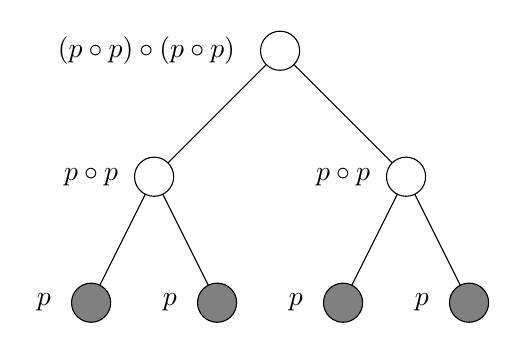
\begin{tikzpicture}[scale=0.8]

    \draw  (1,-1) -- (2,1);
    \draw  (3,-1) -- (2,1);
   \draw  (2,1) -- (4,3);
    \draw  (5,-1) -- (6,1);
    \draw  (7,-1) -- (6,1);
    \draw  (6,1) -- (4,3);

    \node[shape=circle, draw=black, fill = white, scale = 1.5]  at (4,3) {};
    \node[shape=circle, draw=black, fill = white, scale = 1.5]  at (2,1) {};
    \node[shape=circle, draw=black, fill = gray, scale = 1.5]  at (1,-1) {};
    \node[shape=circle, draw=black, fill = gray, scale = 1.5]  at (3,-1) {};
    \node[shape=circle, draw=black, fill = white, scale = 1.5]  at (6,1) {};
    \node[shape=circle, draw=black, fill = gray, scale = 1.5]  at (5,-1) {};
    \node[shape=circle, draw=black, fill = gray, scale = 1.5]  at (7,-1) {};

    \node at (1/4,-1) {$p$};
    \node at (9/4,-1) {$p$};
    \node at (17/4,-1) {$p$};
    \node at (25/4,-1) {$p$};
    \node at (1,1) {$p \circ p$};
    \node at (20/4,1) {$p \circ p$};
    \node at (8/4,3) {$(p\circ p) \circ (p \circ p)\;\;$};


\end{tikzpicture}
\end{subfigure}
\hspace{2 cm}
\begin{subfigure}

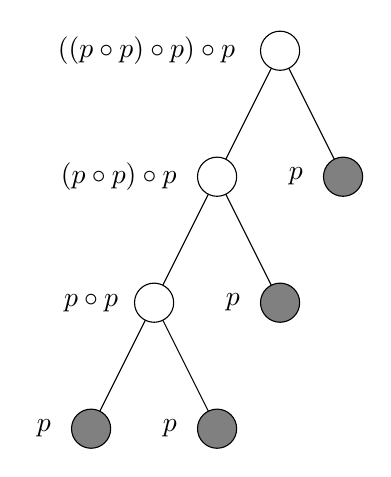
\begin{tikzpicture}[scale=0.8]

    \draw  (1,-3) -- (4,3);
    \draw  (3,-3) -- (2,-1);
    \draw  (4,-1) -- (3,1);
    \draw  (5,1) -- (4,3);

    \node[shape=circle, draw=black, fill = white, scale = 1.5]  at (3,1) {};
    \node[shape=circle, draw=black, fill = white, scale = 1.5]  at (2,-1) {};
    \node[shape=circle, draw=black, fill = gray, scale = 1.5]  at (1,-3) {};
    \node[shape=circle, draw=black, fill = gray, scale = 1.5]  at (3,-3) {};
    \node[shape=circle, draw=black, fill = gray, scale = 1.5]  at (4,-1) {};
    \node[shape=circle, draw=black, fill = white, scale = 1.5]  at (4,3) {};
    \node[shape=circle, draw=black, fill = gray, scale = 1.5]  at (5,1) {};

    \node at (1/4,-3) {$p$};
    \node at (9/4,-3) {$p$};
    \node at (1,-1) {$p \circ p$};
    \node at (13/4,-1) {$p$};
    \node at (17/4,1) {$ p$};
    \node at (6/4,1) {$(p\circ p) \circ p\;$};
    \node at (8/4,3) {$((p\circ p) \circ p)\circ p\;\;$};



\end{tikzpicture}
\end{subfigure}
\caption{Two possible trees $\g,\g'\in\G(4)$, and the corresponding distributions $C_{\gamma}(p) = (p\circ p) \circ (p \circ p)$ and $C_{\gamma'}(p) = ((p\circ p) \circ p)\circ p.$}\label{fig1}
\end{figure}



For example, if $k=3$, there are only two trees $\g,\g'\in\G(3)$, with $\a_3(\g)=\a_3(\g')=1/2$ and
\begin{align}\label{eq2}
C_{\gamma}(p)=(p \circ p)\circ p=p\circ(p \circ p)= C_{\gamma'}(p).
\end{align}
We refer to Figure~\ref{fig1} for two examples of $C_{\gamma}(p)$ for $\g\in\G(4)$.


Since each collision is of the form $q\circ q'$ for some $q,q'\in\cP(\O)$ and since by~\eqref{defconv1} one has
\begin{align}\label{lab:nons}
&p \circ q = \sum_{A\,\subset\,[n]}\bar\nu(A)\,p_A \otimes q_{A^c},
\end{align}
where $\bar\nu(A)= \frac12(\nu(A)+\nu(A^c))$, one can write the following expansion for the resulting measure at the root:
\begin{align}\label{eq5}
C_{\gamma}(p)= \sum_{\vec A\,\in\,\cV_n^{k-1}}\nu(\vec A) C^{\vec A}_{\gamma}(p),
\end{align}
where $\cV_n$ is the set of subsets of $[n]$, so that $\vec A\in \cV_n^{k-1}$ represents a pattern $\vec A=(A_1,\,\dots,\,A_{k-1})$,
\begin{equation}\label{eq:nua}
\nu(\vec A)= \prod_{i=1}^{k-1}\bar\nu(A_i)
\end{equation}
and $C^{\vec A}_{\gamma}(p)\in\cP(\O)$ is the distribution computed as follows. Each internal node $v_i$, $i=1,\,\dots\,,k-1$, in $\gamma$ (in some fixed order) is associated with the set $A_i$, and we attach the mark $A_i$ to the edge connecting $v_i$ to its left child and the mark $A_i^c$ to the edge connecting $v_i$ to its right child in $\gamma$. In this way we obtain a tree $\gamma$ with marks on all its edges. Let $d_i$ denote the depth of the $i^{\rm th}$ leaf of $\gamma$ (e.g.\ counting from the leftmost leaf), and consider $p_{V_i(\vec A)}$, the marginal of the measure $p$ on the subset
\begin{align}\label{eqa5}
V_i(\vec A):=\cap_{j=1}^{d_i} A^i_j,
\end{align}
where $A^i_1,\dots,A^i_{d_i}$ are the marks encountered along the edges of the unique path from the root to the $i^{\rm th}$ leaf. Then $ C^{\vec A}_{\gamma}(p)$ is given by
\begin{align}\label{eq6}
C^{\vec A}_{\gamma}(p) = p_{V_1(\vec A)}\otimes\cdots\otimes p_{V_k(\vec A)}.
\end{align}
Note that some of the $V_i(\vec A)$ may be empty. However, they form a partition of $[n]$, namely $V_i(\vec A)\cap V_j(\vec A)=\emptyset$ for $i\neq j$ and $\cup_{i=1}^kV_i(\vec A)=[n]$, which can be seen as the result of a fragmentation process
\[
[n]\to (A_1,A_1^c) \to (A_1\cap A_2,A_1\cap A_2^c,A_1^c)\to\cdots\to \left(V_1(\vec A),\cdots,V_k(\vec A)\right).
\]
As an example, in the case~\eqref{eq2} we have $\vec A=(A_1,A_2)$, and
\begin{align}
(p \circ p)\circ p = \sum_{A_1,\,A_2 \,\subset\,[n]}\bar\nu(A_1)\bar\nu(A_2)p_{A_1\,\cap\,A_2}\otimes p_{A_1\,\cap\,A_2^c} \otimes p_{A_1^c}.
\end{align}
The proof of~\eqref{eq00}-\eqref{eq5} can be easily done by induction, by splitting the tree $\g\in\G(k)$ into the left and right subtrees $\g_l,\g_r$ and using the relation~\eqref{eqreca}, see the proof of~\eqref{eq:idto} below for a closely related explicit computation.

In conclusion, from~\eqref{wildsums}, \eqref{eq00} and~\eqref{eq5} we obtain the following representation of the distribution $p_t$ as a convex combination of distributions $C^{\vec A}_{\gamma}(p)$:
\begin{align}\label{eq0}
p_t=\sum_{k=1}^{\infty}\b_t(k)\sum_{\g\,\in \,\Gamma(k)}\alpha_k(\g)\sum_{\vec A\,\in\, \cV_n^{k-1}}\nu(\vec A) \,C^{\vec A}_{\gamma}(p),
\end{align}
where $\b_t(k) := e^{-t}(1-e^{-t})^{k-1}$ is a probability on $\bbN$ for each $t\geq 0$, $ \alpha_k(\g)$ is a probability on $\G(k)$ for all $k$, and $\nu(\vec A)$ is a probability on $\cV_n^{k-1}$ for all $k$.

\begin{theorem}\label{contrlemma2}
For any probability measure $p,q \in \cP(\O)$ such that $p_{i} = q_{i}$ for all $i \in [n]$, all $t\geq 0$,
\begin{align}\label{nonlincont1}
\|S_t(p)-S_t(q)\|_\tv \leq \tfrac12\,n(n-1)\,\|p-q\|_\tv \,e^{-D(\nu) t}
\end{align}
where $D(\nu)=1-r(\nu)$.
\end{theorem}

\begin{proof}
From~\eqref{eq0} we write
\begin{align}\label{eqb17}
S_t(p) - S_t(q) =\sum_{k=1}^\infty \b_t(k) s^{(k)},
\end{align}
where
\begin{align}\label{eqba17}
s^{(k)}=\sum_{\gamma\,\in\,\Gamma(k)}\alpha_k(\gamma)
\sum_{\vec A\,\in\,\cV_n^{k-1}}\nu(\vec A) \,\left[C^{\vec A}_{\gamma}(p)-C^{\vec A}_{\gamma}(q)\right]\,.
\end{align}
We introduce some further notation in order to handle more explicitly the difference of probability measures $C^{\vec A}_{\gamma}(p)-C^{\vec A}_{\gamma}(q)$. For any given $\g\in\G(k)$, and $\vec A\in \cV_n^{k-1}$, $\phi:\O\mapsto\bbR$, we may write
\begin{multline}\label{eqb28}
\scalar{C^{\vec A}_{\gamma}(p)-C^{\vec A}_{\gamma}(q)}{\phi}\\
 =\sum_{(x,y)\,\in\,\Omega^k\,\times\, \Omega^k}\mu(x,y) \sum_{z\,\in\,\Omega} \phi(z)\left(\ind\left(z=u(y,\vec A)\right)-\ind\left(z=u(x,\vec A)\right)
\right)
\end{multline}
where $x=(x^i,i=1,\,\dots,\,k)\in\O^k$ stands for the configurations sampled with $q^{\otimes k}$ over the leaves of $\g$, $y=(y^i,i=1,\,\dots,\,k)\in\O^k$ stands for the configurations sampled with $p^{\otimes k}$ over the leaves of $\g$, and $\mu(x,y)=\prod_{i=1}^k\mu_1(x^i,y^i)$ denotes a coupling of these two product measures, such that for every $i=1,\,\dots,\,k$, $\mu_1(x^i,y^i)$ is the optimal coupling of $(q,p)$:
\begin{align}\label{eq29}
\|p-q\|_{\tv} = \sum_{(x,y)\,\in\,\Omega^k\,\times\,\Omega^k}\mu(x,y) \ind\left(x^i\neq y^i\right)=\sum_{x^i,y^i\,\in\,\Omega}\mu_1\left(x^i,y^i\right) \ind\left(x^i\neq y^i\right).
\end{align}
The notation $u(x,\vec A)$ in~\eqref{eqb28} is defined as follows. Note that $x^i\in\O$ is a vector $x^i=(x^i_1,\,\dots,\,x^i_n)$, for every $i$, with $x^i_\ell\in\{0,\,\dots,\,q_\ell\}$, and write $x^i_A=(x^i_\ell)_{\ell\,\in\,A}$ for the content of $x^i$ on $A\subset[n]$. With this notation, given $x\in\Omega^k$ and $\vec A\in\cV_n^{k-1}$, $u(x,\vec A)\in\O$ is defined as the unique configuration such that
\[
u(x,\vec A)_{V_i(\vec A)} = x^i_{V_i(\vec A)}
\]
for every $i=1,\,\dots,\,k$. In words, for each $i\in[k]$, the content of the configuration $u(x,\vec A)$ on the set $V_i(\vec A)\subset V$ is taken from the configuration $x^i$ at the $i^{\rm th}$ leaf. The validity of~\eqref{eqb28} is thus a consequence of~\eqref{eq6}.

Let $\partial\g$ denote the set of leaves of $\g$. Notice that
\begin{gather*}
\ind(z=u(x,\vec A)) =
\prod_{i\,\in\,\partial \g}
\ind(z_{V_i(\vec A)}=x^i_{V_i(\vec A)})
\end{gather*}
Let $F=F(\vec A,\g)\subset \partial \g$ denote the set of leaves $i\in \partial \g$ such that $|V_i(\vec A)|> 1$, and write
\[
\ind(z=u(x,\vec A)) = w_F (x,z,\vec A) w_{F^c}(x,z,\vec A)\,,
\]
where for any $S\subset \partial \g$ we write
\begin{equation}\label{defwS}
w_S(x,z,\vec A) = \prod_{i\,\in\,S}
\ind(z_{V_i(\vec A)}=x^i_{V_i(\vec A)}).
\end{equation}
We write $X=(X^i)_{i=1,\,\dots,\,k}$ and $Y=(Y^i)_{i=1,\,\dots,\,k}$ for the random variables with distribution $q^{\otimes k}$ and $p^{\otimes k}$ respectively. Using the fact that $\mu$ is a product over the leaves, and the fact that $p,q$ have the same marginals, for fixed $z\in\O$ we have
\begin{align}\label{eq282a}
\begin{split}
\mu\left[w_{F^c} \left(X,z,\vec A\right)\right]&=\sum_{(x,y)}\mu(x,y) \prod_{i\,\in\, F^c}
\ind\left(z_{V_i(\vec A)}=x^i_{V_i(\vec A)}\right) \\
&= \sum_{(x,y)}\mu(x,y) \prod_{i\,\in\,F^c}
\ind\left(z_{V_i(\vec A)}=y^i_{V_i(\vec A)}\right) =
\mu\left[w_{F^c} (Y,z,\vec A)\right],
\end{split}
\end{align}
and
\begin{align}\label{eq282}
\begin{split}
\mu\left[w_{\partial \g}\left(Y,z,\vec A\right)\right]&=\sum_{(x,y)}\mu(x,y)
\ind\left(z=u(y,\vec A)\right)\\
&=\mu\left[w_{F^c} \left(X,z,\vec A\right)\right]\mu\left[w_F \left(Y,z,\vec A\right)\right].
\end{split}
\end{align}
With this notation we rewrite~\eqref{eqb28} as
\begin{multline}\label{eqbb28}
\left\langle C^{\vec A}_{\gamma}(p)-C^{\vec A}_{\gamma}(q),\phi\right\rangle\\
\begin{aligned}
&=
\sum_{z\,\in\,\Omega} \phi(z) \left[
\mu[w_{\partial \g}\left(Y,z,\vec A\right)] - \mu[w_{\partial \g}\left(X,z,\vec A\right)\right],
\\
&=
\sum_{z\,\in\,\Omega} \phi(z)
\mu\left[w_{F^c} \left(X,z,\vec A\right)\right]\,\mu\left[w_F \left(Y,z,\vec A\right)-w_F \left(X,z,\vec A\right)
\right].
\end{aligned}
\end{multline}
Note that $w_F (Y,z,\vec A)]\neq w_F (X,z,\vec A)$ implies that there exists $i\in F$ such that $X^i\neq Y^i$. Therefore, from~\eqref{eq29} we see that
\begin{multline}\label{eqbb2a8}
\sum_{z\,\in\,\Omega} \mu
\left[w_{F^c} \left(X,z,\vec A\right)\right]\,
\left|\mu
\left[w_F \left(Y,z,\vec A\right)-w_F \left(X,z,\vec A\right)
\right]\right|\\
\begin{aligned}
&\leq
\sum_{i\,\in\,F}\sum_{z\,\in\,\Omega} \mu\left[w_{F^c} \left(X,z,\vec A\right)\right]\,\mu\left[\left|w_F \left(Y,z,\vec A\right)-w_F \left(X,z,\vec A\right)\right|\ind\left(X^i\neq Y^i\right)
\right] \\
&\leq 2\sum_{i\,\in\,F}
\mu\left[X^i\neq Y^i
\right] = 2|F|\,\|p-q\|_\tv.
\end{aligned}
\end{multline}
Therefore, we have shown that~\eqref{eqba17} satisfies
\begin{align}\label{eq2aa86}
& \left|\left\langle s^{(k)},\phi\right\rangle\right|\leq 2\,\|\phi\|_\infty\,\|p-q\|_\tv \sum_{\gamma\,\in\,\Gamma(k)}\alpha_k(\gamma)
\sum_{\vec A\,\in\,\cV_n^{k-1}}\nu(\vec A)\,|F|.
\end{align}
To estimate~\eqref{eq2aa86}, let us call $\cA_{j}=\cA_j(\gamma)$ the set of $\vec A\in\cV_n^{k-1}$ such that $|V_j(\vec A)|\geq 2$, and let $\cA=\cup_{j=1}^k\cA_j$. If $\vec A\notin\cA$ then all sets $V_j(\vec A)$ are either empty or a single site and therefore $|F|=0$. Moreover, $|F|=\sum_{j=1}^k\ind(\cA_{j})$. Therefore we write
\begin{align}
\sum_{\vec A\,\in\,\cV_n^{k-1}}\nu(\vec A)\,|F|= \sum_{j=1}^k
\nu(\cA_j).
\end{align}
To estimate the probability $\nu(\cA_j)$, observe that the event $\cA_j$ implies that there exists $i_1<i_2\in[n]$ such that $\{i_1,i_2\} \in V_j(\vec A)$. Moreover, recalling~\eqref{eqa5},
\begin{align*}
\nu\left(\{i_1,i_2\} \in V_j(\vec A)\right)& = \nu\left(\{i_1,i_2\} \in \cap_{l=1}^{d_j} A^j_l\right) = \bar \nu\left(\{i_1,i_2\} \in A\right)^{d_j}
\leq \left(\frac{r(\nu)}{2}\right)^{d_j},
\end{align*}
where we use the fact that for any $i_1<i_2$, the probability under $\bar\nu$ that $\{i_1,i_2\} \in A$ is bounded by $r(\nu)/2$. Indeed, conditionally on not being separated the probability that both $i_1,i_2$ belong to $A$ under $\bar\nu$ is $1/2$ by symmetry. A union bound then shows that
\[
\nu(\cA_j)\leq \tfrac12\,n(n-1)\left(\frac{r(\nu)}{2}\right)^{d_j}.
\]
In conclusion, if we define
\begin{align}\label{eqomegagamma}
\o(\gamma):=\sum_{j=1}^k\left(\frac{r(\nu)}{2}\right)^{d_j},
\end{align}
we obtain, for all $k\in\bbN$,
\begin{align}\label{eq10}
& \left|\left\langle s^{(k)},\phi\right\rangle\right|\leq{n(n-1)}\,\|\phi\|_\infty\,\|p-q\|_\tv \sum_{\gamma\,\in\,\Gamma(k)}\alpha_k(\gamma)
\,\o(\g).
\end{align}
From~\cite[Lemma~1.4]{carlenwild}, one has, for all $\e>0$,
\begin{align}\label{carlenwildestimation}
\sum_{\gamma\,\in\,\Gamma(k)}\alpha_k(\gamma)\o(\gamma) \leq B_\e e^{-a_\e\log k}.
\end{align}
with $a_\e=(1-r(\nu))/(1+\e)$ and $B_\e=B_\e(r(\nu),\e)$. One could use this estimate to obtain an almost optimal decay rate $a_\e$. However, here we obtain the optimal exponential decay rate by computing the expectation of $\o(\g)$.

\begin{lemm}\label{lemma:omega}
For any $t\geq 0$,
\begin{equation}\label{lem:omega}
\sum_{k=1}^{\infty}\b_t(k)\sum_{\g\,\in \,\Gamma(k)}\alpha_k(\g)\,\o(\gamma) = e^{-(1-r(\nu))t}.
\end{equation}
\end{lemm}

Assuming the validity of~\eqref{lem:omega}, and using $\|\mu-\mu'\|_\tv = \tfrac12 \max_{f:\,\|f\|_\infty\leq 1} |\mu(f)-\mu'(f)|$, from~\eqref{eqb17} and~\eqref{eq10} we obtain
\begin{align}\label{eqabb17}
\|S_t(p) - S_t(q)\|_\tv
\leq \tfrac12\,n(n-1)\,\|p-q\|_\tv \,e^{-(1-r(\nu))t},
\end{align}
which concludes the proof of Theorem~\ref{contrlemma2}.

It remains to prove~\eqref{lem:omega}. For any $\g\in\cup_{k=1}^\infty\G(k)$, define $\bbP_t(\g) = \b_t(k)\alpha_k(\g)$, where $k$ is such that $\g\in\G(k)$. Notice that for any $\g\in\cup_{k=1}^\infty\G(k)$,
\begin{equation}\label{lem:omega1}
\bbP_t(\g) = \ind_{\g=\emptyset}\,e^{-t} + \ind_{\g\neq \emptyset}\int_0^t e^{-s}\bbP_{t-s}(\g_l)\bbP_{t-s}(\g_r)ds,
\end{equation}
where $\emptyset$ denotes the empty tree with one leaf (given by the root), while for $\g\neq \emptyset$ we write $\g_l,\g_r$ for the left and right subtrees. Indeed, for $\g=\emptyset$~\eqref{lem:omega1} is immediate, while for $\g\neq\emptyset$, supposing $\g\in\G(k)$, and recalling~\eqref{eqreca} one has
\begin{align*}
\bbP_{t}(\g) &= e^{-t}\left(1-e^{-t}\right)^{k-1}\a_k(\g) = e^{-t}\int_0^{t}e^{-(t-s)}\left(1-e^{-(t-s)}\right)^{k-2}(k-1)\a_k(\g)ds\\ &=
\int_0^t e^{-s}e^{-2(t-s)}\left(1-e^{-(t-s)}\right)^{k-2}\a_j(\g_l)\a_{k-j}(\g_r)ds =\int_0^t e^{-s} \bbP_{t-s}(\g_l)\bbP_{t-s}(\g_r)ds.
\end{align*}
To prove Lemma~\ref{lemma:omega}, note that the left hand side of~\eqref{lem:omega} is given by $\sum_\g \bbP_t(\g)\o(\g)$. Using~\eqref{lem:omega1} and $\o(\emptyset)=1$, we see that
\begin{align*}
\z(t):&=\sum_\g\bbP_{t}(\g)\o(\g) =e^{-t} +\frac{r(\nu)}2
\sum_{\g\neq\emptyset}\int_0^t e^{-s} \bbP_{t-s}(\g_l)\bbP_{t-s}(\g_r)(\o(\g_l)+\o(\g_r))ds\\
&=e^{-t} +r(\nu)
\sum_{\g}\int_0^t e^{-s} \bbP_{t-s}(\g)\o(\g)ds=e^{-t} +r(\nu)
\int_0^t e^{-s} \z(t-s)ds.
\end{align*}
Differentiating, and integrating by parts the resulting expression one finds $\dot\z(t) = -(1-r(\nu))\z(t)$. Since $\z(0)=1$ we obtain $\z(t)=e^{-(1-r(\nu))t}$, $t\geq 0$.
\end{proof}

\subsection{Contraction for the linearized equation}

Consider the symmetric bilinear form $\hat{Q}(f,g)$ defined by
\begin{multline}
 \hat{Q}(f,g)(\eta)\\
=
\frac{1}{2}\sum_{A,\si}
\nu(A)\big(f(\sigma_{A} \eta_{A^c}) g(\eta_{A}\sigma_{A^c}) + g(\sigma_{A} \eta_{A^c})f(\eta_{A}\sigma_{A^c}) - f(\sigma)g(\eta)- g(\sigma)f(\eta)\big),
\end{multline}
where $\eta \in \Om$, $f,g:\O\mapsto\bbR$, and the sum extends to all $A \subset [n]$ and $\si \in \O$.
If $p \in \cP(\O)$, then $\hat{Q}(p,p) = Q(p),$ where
\[
Q(p)=\sum_A\nu(A)(p_A\otimes p_{A^c} - p)
\]
is the generator associated to~\eqref{boltzeq}, that is the non linear semigroup $\{S_t, t \geq 0\}$ satisfies $S_0 (p)= p$ and $\partial_t S_t (p)= Q (S_t (p))$, $t\geq 0$.
Next, consider the differential equation
\begin{align}\label{linsem}
&\partial_t h_t = 2\hat{Q}(q_t,h_t), \ \ \ \;\;\; h_0=h,
\end{align}
where $q_t = S_t(q)$ for some fixed $ q \in \cP(\O)$. Note that it is linear in $h$.
We write its unique solution as
\[
h_t=\bar{S}_t(q)(h),
\]
that is $\bar{S}_t(q)(h)$ verifies $\partial_t \bar{S}_t(q)(h) = 2\hat{Q}(q_t,\bar{S}_t(q)(h))$, $\bar{S}_0(q)(h)=h$ and

Our main result concerning the linearized equation reads as follows.

\begin{theo}\label{wasscontrlemma2}
For all $p,q \in \cP(\O)$ such that $p_{i} = q_{i}$ for all $i \in [n]$, and $\phi:\O\mapsto\bbR$, for all $t>0$,
\begin{equation}\label{nonlincont2}
\left\langle \bar{S}_t(q)(p-q),\phi\right\rangle  \leq n(n-1)\|\phi\|_{\infty}e^{-D(\nu) \,t}\,\|p-q\|_\tv,
\end{equation}
\begin{multline}\label{nonlincont3}
\left\langle S_t(p)-S_t(q)-\bar{S}_t(q)(p-q),\phi\right\rangle \\
\leq \frac1{16}\,n^3(n-1)(n-2) \|\phi\|_{\infty}e^{-D(\nu) \,t}\,\|p-q\|_\tv^2, 
\end{multline}
where $D(\nu)= 1-r(\nu)$.
\end{theo}

The proof of Theorem~\ref{wasscontrlemma2} requires several steps. We start by giving an explicit representation of the solution $\bar{S}_t(q)(p-q)$ to~\eqref{linsem} when $h=p-q$. To this end let us define, for any $k\geq 2$, $\g\in\G(k)$, the distribution $C_{\gamma, p}(q)$ as the measure defined in~\eqref{eq5} with the only difference that we take the distribution $p$ instead of $q$ at the rightmost leaf of $\g$, all other leafs remaining with the distribution $q$. Formally,
\begin{align}\label{eqab5}
C_{\gamma,p}(q)= \sum_{\vec A\,\in\,\cV_n^{k-1}}\nu(\vec A) \,C^{\vec A}_{\gamma,p}(q),\qquad C^{\vec A}_{\gamma,p}(q) = q_{V_1(\vec A)}\otimes\cdots\otimes q_{V_{k-1}(\vec A)}\otimes p_{V_{k}(\vec A)}.
\end{align}


In what follows we denote by $d_r(\g)$ the depth of the rightmost leaf in $\g$.

\begin{lemm}\label{lem:wildrep}
For all $p,q \in \cP(\O)$, $t\geq 0$,
\begin{align}\label{eq:topid}
\bar{S}_t(q)(p-q) = \sum_{k=1}^\infty\b_t(k) \sum_{\gamma\,\in\,\Gamma(k)}\alpha_k(\gamma)\left(C_{\gamma, p}(q)-C_{\gamma}(q)\right)2^{d_r(\gamma)}.
\end{align}
\end{lemm}

\begin{proof}
Fix $p,q \in \cP(\O)$. If $h_t=\bar{S}_t(q)(p)$, then
\begin{align*}
\partial_t \sum_{\sigma}h_t(\sigma) = 2\sum_{\sigma}\hat{Q}(q_t,h_t)(\si) = 0.
\end{align*}
Thus $ \sum_{\sigma}h_t(\sigma) = 1$, and $2\hat{Q}(q_t,h_{t})=2q_t \circ h_{t} - q_t - h_{t}$. Therefore $h_t$ satisfies
\begin{align}
h_t = qe^{-t} + \int_{0}^te^{-(t-s)}\left(2q_{s} \circ h_{s}-q_{s}\right)ds.
\end{align}
By linearity, $ \bar{S}_t(q)(p-q) =\bar{S}_t(q)(p) - \bar{S}_t(q)(q)$ satisfies $\bar{S}_t(q)(p-q) =u_t-v_t$, where
\begin{align}\label{eq:solve}
u_t = pe^{-t} + \int_{0}^te^{-(t-s)}2q_{s} \circ u_{s}ds,\qquad v_t = qe^{-t} + \int_{0}^te^{-(t-s)}2q_{s} \circ v_{s}ds.
\end{align}
Wild's construction then shows that
\begin{align}\label{eq:defuv}
u_t = e^{-t}\sum_{k=1}^{\infty}\left(1-e^{-t}\right)^{k-1}u^{(k)},\qquad v_t = e^{-t}\sum_{k=1}^{\infty}\left(1-e^{-t}\right)^{k-1}v^{(k)},
\end{align}
where $u^{(1)}= p$, $v^{(1)}= q$, and for $k\geq 2$,
\begin{align*}
u^{(k)}= \frac{1}{k-1}\sum_{j=1}^{k-1}2q^{(j)}\circ u^{(k-j)} \,,\qquad v^{(k)}= \frac{1}{k-1}\sum_{j=1}^{k-1}2q^{(j)}\circ v^{(k-j)}.
\end{align*}
respectively, and $q^{(j)}$ is defined by~\eqref{eq:wildp} with $p$ replaced by $q$. To check that this representation of the solution holds, let $u_t$ be defined by~\eqref{eq:defuv}. Then
\begin{align}\label{eq:defuv1}
\begin{split}
\int_{0}^te^{-(t-s)}2q_{s} \circ u_{s}ds &= \sum_{\ell,k=1}^{\infty}
\int_{0}^t\b_s(k)\b_s(\ell)e^{-(t-s)}2q^{(\ell)} \circ u^{(k)}ds\\
& =\sum_{\ell\,<\,k}
\int_{0}^te^{-2s}\left(1-e^{-s}\right)^{k-2}e^{-(t-s)}2q^{(\ell)} \circ u^{(k-\ell)}ds\\
& =\sum_{k\,\geq\,2}
\int_{0}^t(k-1)e^{-s}\left(1-e^{-s}\right)^{k-2}e^{-t} u^{(k)}ds \\
& =\sum_{k\,\geq\,2} \left(1-e^{-t}\right)^{k-1}e^{-t} u^{(k)} = u_t - e^{-t} u^{(1)} = u_t - e^{-t} p.
\end{split}
\end{align}
Thus $u_t$ solves~\eqref{eq:solve}. The same applies to $v_t$. This proves~\eqref{eq:defuv}.

Next, we prove that
\begin{align}\label{eq:idto}
u^{(k)}=\sum_{\gamma\,\in\,\Gamma(k)}\alpha_k(\gamma)C_{\gamma,p}(q)2^{d_r(\gamma)}\,,\qquad v^{(k)}=\sum_{\gamma\,\in\,\Gamma(k)}\alpha_k(\gamma)C_{\gamma}(q)2^{d_r(\gamma)}
\end{align}
for all $k \geq 2$. Let us prove this by using induction over $k$. If $k=2$ then $u^{(2)} = 2 q\circ p$ and thus the claimed identity holds. If the formula holds for $j \leq k-1,$ then using~\eqref{eq5} and~\eqref{eqreca},
\begin{align*}
u^{(k)}&=\frac{1}{k-1}\sum_{j=1}^{k-1}2q^{(j)}\circ u^{(k-j)} \\
&=\frac{1}{k-1}\sum_{j=1}^{k-1}\sum_{\substack{\gamma_l\,\in\,\Gamma(j) \\ \gamma_r\,\in\,\Gamma(k-j)}}\alpha_j(\gamma_l)\alpha_{k-j}(\gamma_r) C_{\gamma_l}(q) \circ C_{\gamma_r, p}(q)2^{d_r(\gamma_r)+1} \\
&=\sum_{\gamma\,\in\,\Gamma(k)}\alpha_k(\gamma)C_{\gamma,p}(q)2^{d_r(\gamma)}.
\end{align*}
This proves the identity~\eqref{eq:idto} for $u$, and the same argument proves the one for $v$. The identities~\eqref{eq:defuv} and~\eqref{eq:idto} imply~\eqref{eq:topid}.
\end{proof}

Next, for any $k\geq 2$, $\g\in\G(k)$, $j\in[k]$, we define
\begin{align}\label{eq11}
C_{\gamma,p,j}(q)= \sum_{\vec A\,\in\, \cV_n^{k-1}}\nu(\vec A) C^{\vec A}_{\gamma,p,j}(q)\,,\qquad C^{\vec A}_{\gamma,p,j}(q):= p_{V_j(\vec A)} \otimes _{\ell\neq j} q_{V_\ell(\vec A)},
\end{align}
which denotes the distribution obtained from the tree $\gamma\in\G(k)$ when all leaves are given the distribution $q$ except for the $j^{\rm th}$ leaf which takes the distribution $p$. When $j=k$, that is $j$ is the rightmost leaf, then we have $C_{\gamma,p,k}(q) = C_{\gamma,p}(q)$.

\begin{lemm}\label{lem:dr}
For any $k\geq 2$, for all $p,q$:
\begin{align}\label{eq18}
\sum_{\gamma\,\in\,\Gamma(k)}\alpha_k(\gamma)2^{d_r}C_{\gamma,p}(q) =\sum_{j=1}^k\sum_{\gamma\,\in\,\Gamma(k)}\alpha_k(\gamma)C_{\gamma,p,j}(q)
\,.
\end{align}
\end{lemm}

\begin{proof}
By symmetry, it holds for $k=2$, since in this case~\eqref{eq18} says $2q\circ p = q\circ p+p\circ q$. Assume that~\eqref{eq18} holds for all $j\leq k-1$. Then
\begin{multline}\label{eq19}
\sum_{\gamma\,\in\,\Gamma(k)}\alpha_k(\gamma)2^{d_r(\gamma)}C_{\gamma,p}(q)\\
\begin{aligned}
&= \frac2{k-1}\sum_{j=1}^{k-1}
\sum_{\gamma\,\in\,\Gamma(j)}\alpha_j(\gamma)C_{\gamma}(q)\circ\left(
\sum_{\gamma'\,\in\,\Gamma(k-j)}\alpha_{k-j}(\gamma')2^{d_r(\gamma')}C_{\gamma',p}(q) \right)\\
& =
\frac2{k-1}\sum_{j=1}^{k-1}\sum_{\gamma\,\in\,\Gamma(j)}\alpha_j(\gamma)C_{\gamma}(q)\circ\left(
\sum_{i=1}^{k-j}\sum_{\gamma'\,\in\,\Gamma(k-j)}\alpha_{k-j}(\gamma')C_{\gamma',p,i}(q) \right)\\
& = 2
\sum_{\gamma\,\in\,\Gamma(k)}\alpha_k(\gamma)\sum_{i=j(\gamma)+1}^{k}C_{\gamma,p,i}(q),
\end{aligned}
\end{multline}
where $j(\gamma)$ is the number of leaves in the left subtree of $\gamma$, and we have used~\eqref{eqreca}. By symmetry,
\begin{align}\label{eq201}
\sum_{\gamma\,\in\,\Gamma(k)}\alpha_k(\gamma)\sum_{i=j(\gamma)+1}^{k}C_{\gamma,p,i}(q) =
\sum_{\gamma\,\in\,\Gamma(k)}\alpha_k(\gamma)\sum_{i=1}^{j(\gamma)}C_{\gamma,p,i}(q)\,.
\end{align}
Therefore,
\begin{multline}\label{eq202}
2
\sum_{\gamma\,\in\,\Gamma(k)}\alpha_k(\gamma)\sum_{i=j(\gamma)+1}^{k}C_{\gamma,p,i}(q)\\
\begin{aligned}
&=
\sum_{\gamma\,\in\,\Gamma(k)}\alpha_k(\gamma)\sum_{i=1}^{j(\gamma)}C_{\gamma,p,i}(q) +\sum_{\gamma\,\in\,\Gamma(k)}\alpha_k(\gamma)\sum_{i=j(\gamma)+1}^{k}C_{\gamma,p,i}(q) \\
& =
\sum_{i=1}^k\sum_{\gamma\,\in\,\Gamma(k)}\alpha_k(\gamma)C_{\gamma,p,i}(q).
\end{aligned}
\end{multline}
The desired identity follows from~\eqref{eq19} and~\eqref{eq202}.
\end{proof}

We can now turn to the proof Theorem of~\ref{wasscontrlemma2}.

\begin{proof}[{\bf Proof of~\eqref{nonlincont2}}]
From Lemma~\ref{lem:wildrep} and Lemma~\ref{lem:dr}, we write
\begin{align}\label{eqbi17}
\bar S_t(q)(p-q) =\sum_{k=1}^\infty \b_t(k) \,\bar s^{(k)},
\end{align}
where
\begin{align}\label{eqbia17}
\bar s^{(k)}=\sum_{j=1}^k\sum_{\gamma\,\in\,\Gamma(k)}\alpha_k(\gamma)
\sum_{\vec A\,\in\,\cV_n^{k-1}}\nu(\vec A) \,\left[C^{\vec A}_{\gamma,p,j}(q)-C^{\vec A}_{\gamma}(q)\right]\,.
\end{align}
Let $\cA_{j}$ denote the set of $\vec A\in\cV_n^{k-1}$ such that $|V_j(\vec A)|\geq 2$. Since $p,q$ have the same marginals, arguing as in the proof of Theorem~\ref{contrlemma2}, we obtain, or all $\phi:\O\mapsto\bbR$,
\begin{align}\label{eqbas17}
\left|\left\langle C^{\vec A}_{\gamma,p,j}(q)-C^{\vec A}_{\gamma}(q), \phi\right\rangle\right|\leq 2\|\phi\|_\infty \|p-q\|_\tv\, \ind(\cA_j)\,.
\end{align}
Therefore, as in~\eqref{eq10} we obtain
\begin{align}\label{eqbas18}
\left|\left\langle \bar s^{(k)},\phi\right\rangle\right|\leq {n(n-1)}\,\|\phi\|_\infty\,\|p-q\|_\tv
\sum_{\gamma\,\in\,\Gamma(k)}\alpha_k(\gamma)
\o(\g).
\end{align}
From~\eqref{eqbi17} and Lemma~\ref{lemma:omega} we conclude the proof of~\eqref{nonlincont2}.
\end{proof}

\begin{proof}[{\bf Proof of~\eqref{nonlincont3}}]
The proof of~\eqref{nonlincont3} requires a bit more work.
Let us define
\[
r_t: = S_t(p) - S_t(q) - \bar{S}_t(q)(p-q).
\]
From Lemma~\ref{lem:wildrep} and Lemma~\ref{lem:dr} we see that
\begin{align}\label{eqa17}
r_t=\sum_{k=1}^\infty \b_t(k) r^{(k)},
\end{align}
where
\begin{align}\label{eqaa17}
r^{(k)}=\sum_{\gamma\,\in\,\Gamma(k)}\alpha_k(\gamma)\left[C_{\gamma}(p)-C_{\gamma}(q)-\sum_{i=1}^k\left(C_{\gamma,p,i}(q)-C_{\gamma}(q)\right)\right]\,,
\end{align}
We are going to prove that for any $\phi:\Omega\mapsto\bbR$,
\begin{align}\label{eq27}
\left\langle r^{(k)},\phi\right\rangle &
\leq \tfrac1{16}\,n^3(n-1)(n-2)\|\phi\|_\infty \|p-q\|^2_{\tv}\sum_{\gamma\,\in\,\Gamma(k)}\alpha_k(\gamma)\o(\g).
\end{align}
By the argument in~\eqref{eqabb17} and Lemma~\ref{lemma:omega} this is sufficient to end the proof.

With the notation from the proof of Theorem~\ref{contrlemma2} we write
\begin{multline}\label{eq28}
\left\langle r^{(k)},\phi\right\rangle=\sum_{\gamma\,\in\,\Gamma(k)}\alpha_k(\gamma)
\sum_{(x,y)\,\in\,\Omega^k\times \Omega^k}\sum_{\vec A\,\in\,\cV_n^{k-1}}\mu(x,y)\nu(\vec A)  \\
\times \sum_{z\,\in\,\Omega} \phi(z)\left(\ind\left(z=u(y,\vec A)\right)-\ind\left(z=u(x,\vec A)\right) 
\right.\\
\left. - \sum_{i=1}^k\left(\ind\left(z=u(x,y,\vec A,i\right) -\ind\left(z=u(x,\vec A)\right) \right)\right),
\end{multline}
where we call $u(x,y,\vec A,j)$ the unique configuration in $\Omega$ such that
\[
u(x,y,\vec A,j)_{V_j(\vec A)} = y^j_{V_j(\vec A)}\,,\qquad u(x,y,\vec A,j)_{V_i(\vec A)} = x^i_{V_i(\vec A)}\,,\;\;\text{for every }\; i\neq j.
\]
That is, $u(x,y,\vec A,j)$ coincides with $u(x,\vec A)$ except that on $V_j(\vec A)$ its content (if not empty) is taken from $y^j$.
It follows that
\begin{gather*}
\ind\left(z=u(x,\vec A)\right) =
\prod_{i\,\in\,\partial \g}
\ind\left(z_{V_i(\vec A)}=x^i_{V_i(\vec A)}\right)\,,\\
\ind\left(z=u\left(x,y,\vec A,j\right)\right) =\ind\left(z_{V_j(\vec A)}=y^j_{V_j(\vec A)}\right)
\prod_{i\,\in\,\partial \g:\; i\neq j}
\ind\left(z_{V_i(\vec A)}=x^i_{V_i(\vec A)}\right)\,,
\end{gather*}
where $\partial\g$ denotes the set of leaves of $\g$.

As in the proof of Theorem~\ref{contrlemma2}, we let $F=F(\vec A,\g)\subset \partial \g$ denote the set of leaves $i\in \partial \g$ such that $|V_i(\vec A)|> 1$, and recall that since $\mu$ is a product over the leaves, and $p,q$ have the same marginals one has the identities~\eqref{eq282a} and~\eqref{eq282}. With this notation we rewrite~\eqref{eq28} as
\begin{multline}\label{eq2a8}
 \left\langle r^{(k)},\phi\right\rangle =\sum_{\gamma\,\in\,\Gamma(k)}\alpha_k(\gamma)
\sum_{\vec A\,\in\,\cV_n^{k-1}}\;\nu(\vec A)\sum_{z\,\in\,\Omega} \phi(z)\\
 \times \left[
\mu\left[w_{\partial \g}\left(Y,z,\vec A\right)\right] - \mu\left[w_{\partial \g}\left(X,z,\vec A\right)\right]\right.\\
-\left. \sum_{i=1}^k\left(\mu\left[w_{\partial \g}\left(X(i,y),z,\vec A\right)\right] - \mu\left[w_{\partial \g}\left(X,z,\vec A\right)\right]
\right)\right],
\end{multline}
where $X(i,y)\in\O^k$ denotes the vector whose $i^{\rm th}$ component is $Y^i$ while all other components are $X^j$. Moreover, for a given choice of $\g,\vec A, z$, the square bracket in~\eqref{eq2a8} is also equal to
\begin{multline}\label{eq2a81}
\mu\left[w_{\partial \g}\left(Y,z,\vec A\right)\right] - \mu\left[w_{\partial \g}\left(X,z,\vec A\right)\right] \\
- \sum_{i=1}^k\left(\mu\left[w_{\partial \g}\left(X(i,y),z,\vec A\right)\right] - \mu\left[w_{\partial \g}\left(X,z,\vec A\right)\right]
\right) \\
 = \mu\left[w_{F^c} \left(X,z,\vec A\right)\right]\,\,\mu\left[w_F \left(Y,z,\vec A\right)-w_F \left(X,z,\vec A\right)\right.\\
\left. -\sum_{i\,\in\,F}
\left(w_{F}\left(X(i,y),z,\vec A\right) - w_{F}\left(X,z,\vec A\right)
\right)\right].
\end{multline}
In particular, if $\g,\vec A$ are such that $F=F(\g,\vec A)=\emptyset$, then~\eqref{eq2a81} vanishes. Moreover, \eqref{eq2a81} vanishes also when $F$ is a single leaf. Indeed, if e.g.\ $F=\{j\}$, then
\begin{multline}\label{eq2a83}
w_F \left(Y,z,\vec A\right)-w_F \left(X,z,\vec A\right)-\sum_{i\,\in\,F}
\left(w_{F}\left(X(i,y),z,\vec A\right) - w_{F}\left(X,z,\vec A\right)
\right)\\
=w_F \left(Y,z,\vec A\right)- w_{F}\left(X(j,y),z,\vec A\right) = 0.
\end{multline}
Thus, we may restrict to the case of $|F|>1$. Therefore,
\begin{align}\label{eq2a85}
& \left|\left\langle r^{(k)},\phi\right\rangle\right|\leq \|\phi\|_\infty\sum_{\gamma\,\in\,\Gamma(k)}\alpha_k(\gamma)
\sum_{\vec A\,\in\,\cV_n^{k-1}} \nu(\vec A)\ind(|F|>1)
\,\mu\left[\G\left(\g,\vec A,X,Y\right)\right],
\end{align}
where we use the notation
\begin{multline}
\G\left(\g,\vec A,X,Y\right)
= \sum_{z\,\in\,\O} w_{F^c} \left(X,z,\vec A\right)\left|w_F \left(Y,z,\vec A\right)-w_F \left(X,z,\vec A\right)\right. \\
\left. -\sum_{i\,\in\,F}
\left(w_{F}\left(X(i,y),z,\vec A\right) - w_{F}\left(X,z,\vec A\right)
\right)\right|.
\end{multline}
Clearly, if $X=Y$ the expression within absolute values above vanishes. Moreover, the same applies if $(X,Y)$ is such that $X^i=Y^i$ for all $i\in F$ except one leaf $j\in F$ where $X^j\neq Y^j$. Indeed, in this case $X(i,y)=X$ for all $i\in F$, $i\neq j$, and $X(j,y)=Y$. Given $X,Y$ we write $E=E(X,Y)\subset F$ for the set of leaves $i\in F$ where $X^i\neq Y^i$. Then
\begin{multline}\label{abbao}
\G\left(\g,\vec A,X,Y\right)=\sum_z w_{E^c\cup F^c} \left(X,z,\vec A\right)\\
\left|w_E \left(Y,z,\vec A\right)-w_E \left(X,z,\vec A\right)-\sum_{i\,\in\,E}
\left(w_{E}\left(X(i,y),z,\vec A\right) - w_{E}\left(X,z,\vec A\right)\right)\right|\\
 \leq \sum_z w_{E^c} \left(X,z,\vec A\right)\left|w_E \left(Y,z,\vec A\right)-\sum_{i\,\in\,E} w_{E}\left(X(i,y),z,\vec A\right)\right|\\
\ind(|E|>1)+ (|E|-1)\ind(|E|>1)\\
\leq (|E|+1)\ind(|E|>1)+ (|E|-1)\ind(|E|>1) 
\\ = 2|E|\ind(|E|>1) \leq 2|F|\ind(|E|>1).
\end{multline}
Next, we use $|F|\leq n/2$, since $\cup_{i\in F}V_i(\vec A)\subset [n]$ and $|V_i(\vec A)|\geq 2$ for all $i\in F$. Since $\mu$ is a product over leaves and on each leaf it satisfies~\eqref{eq29}, a union bound over the set of pairs in $F$ shows that
\begin{align}\label{eqa128}
\mu\left[|E|>1\right]\leq \tfrac12\,|F|(|F|-1)\|p-q\|_{\tv}^2.
\end{align}
Therefore,
\begin{align}\label{eq2a86}
& \left|\left\langle r^{(k)},\phi\right\rangle\right|\leq \|\phi\|_\infty \|p-q\|_{\tv}^2\sum_{\gamma\,\in\,\Gamma(k)}\alpha_k(\gamma)
\nu\left(|F|^2(|F|-1)\right).
\end{align}
Next, observe that $|F|\leq n/2$, since $\cup_{i\,\in\,F}V_i(\vec A)\subset [n]$ and $|V_i(\vec A)|\geq 2$ for all $i\in F$. Thus, if $|F|>1$ one has $|F|^2(|F|-1)\leq n^2(n-2)/8$. Summarizing,
\begin{align}\label{eq2a87}
\left|\left\langle r^{(k)},\phi\right\rangle\right|\leq \tfrac{1}8\,n^2(n-2)\,\|\phi\|_\infty\,\|p-q\|_{\tv}^2 \sum_{\gamma\,\in\,\Gamma(k)}\alpha_k(\gamma)\nu(|F|>1).
\end{align}
For a given tree $\g$, the argument in~\eqref{eq10} shows that
\[
\nu(|F|>1)
\leq
\nu(|F|\geq 1) \leq
\tfrac12\,n(n-1)\sum_{i=1}^k\left(\frac{r(\nu)}{2}\right)^{d_i(\g)} = \tfrac12\,n(n-1)\,\,\o(\g),
\]
where we use the fact that the event $F\geq 1$ coincides with $\cup_{i=1}^k\cA_i$ from the proof of~\eqref{eq10}. This ends the proof of~\eqref{eq27}, which completes the proof of~\eqref{nonlincont3}.
\end{proof}

\subsection{Monotonicity of \texorpdfstring{$W$}{W} along the nonlinear evolution}

Before proving Theorem~\ref{unifpropchaos}, we show that the distance $W$ appearing in that statement is monotone along the semigroup. We refer to~\cite{tanaka} for a similar argument in the case of kinetic models. It will be convenient to work with a more symmetric version of~\eqref{eq5}. Since $p\circ q = \sum_A \bar\nu(A) (p\circ q)^A$ we may rewrite~\eqref{eq5} as
\begin{align}\label{eq:symme}
C_{\gamma}(p)= \sum_{\vec A\,\in\,\cV_n^{k-1}} \nu(\vec A)
\hat{C}^{\vec A}_{\gamma}(p)
\end{align}
where $\nu(\vec A)$ is defined as in~\eqref{eq:nua}, and $\hat{C}^{\vec A}_{\gamma}(p)$ represents the symmetric convolutions associated to the sampled sets $(A_1,\,\dots,\,A_{k-1})$. In other words, $\hat{C}^{\vec A}_{\gamma}(p)$ is defined recursively by the following relations. If $\gamma \in \Gamma(k)$ then, decomposing $\g$ into the left and right subtrees $\g_l,\g_r$ as in~\eqref{eqreca}, one has
\begin{align}\label{lab:rec}
 \hat{C}^{\vec A}_{\gamma}(p) = \left(\hat{C}^{\vec{A}_{l}}_{\gamma_l}(p)\circ \hat{C}^{\vec{A}_{r}}_{\gamma_r}(p)\right)^{A_1}
\end{align}
where $A_1$ is the set attached to the root, and
\[
\vec{A}_{l} :=\left(A_2,\,\dots,\,A_j\right), \vec{A}_{r} :=\left(A_{j+1},\,\dots,\,A_{k-1}\right)
\]
are the sets associated to the left and right subtrees respectively. For example, in the case where $C_{\gamma}(p) = ((p \circ p)\circ p)\circ p$ as in Figure~\ref{fig1}, one has
\begin{align}
C_{\gamma}(p) = \sum_{A_1,A_2,A_3\,\subset\, [n]}\bar\nu(A_1)\bar \nu(A_2)\bar \nu(A_3)\hat{C}^{A_1,A_2,A_3}_{\gamma}(p)
\end{align}
where $\hat{C}^{A_1,A_2,A_3}_{\gamma}(p) = (((p\, \circ\, p)^{A_3}\circ \,p)^{A_2})\circ\, p)^{A_1}$. Therefore, as in~\eqref{eq0} one obtains the decomposition
\begin{align}\label{eq60}
p_t=\sum_{k=1}^{\infty}\b_t(k)\sum_{\g\,\in \,\Gamma(k)}\alpha_k(\g)\sum_{\vec A\,\in \,\cV_n^{k-1}}\nu(\vec A) \,\hat C^{\vec A}_{\gamma}(p).
\end{align}

\begin{lemm}\label{wasscontrlemma}
For any $p, q \in \cP(\O)$, any $k\in\bbN$, any $\g\in\G(k)$, and any $\vec A\in \cV_n^{k-1}$, one has
\begin{align}\label{eq:mon1}
W\left(\hat C^{\vec A}_{\gamma}(p),\hat C^{\vec A}_{\gamma}(q)\right) \leq W\left(p,q\right).
\end{align}
In particular, $W(S_t(p),S_t(q)) \leq W(p,q)$ for any $t\geq 0$.
\end{lemm}

\begin{proof}
First we show
\begin{align}\label{wildineq1}
W\left((p_1 \circ p_2),(q_1 \circ q_2)\right)\leq \tfrac{1}{2}\,W\left(p_1,q_1\right) + \tfrac{1}{2}\,W\left(p_2,q_2\right)
\end{align}
for all $p_1,p_2,q_1,q_2 \in \cP(\O).$ For a fixed $A \subset [n]$ and configurations $x_1, x_2 \in \Om$ we define
\begin{align*}
\Pi_{x_1,x_2,A}(z) := \tfrac{1}{2}\big(\IND(z_A = x_{1,A}, z_{A^c}=x_{2,A^c})+\IND(z_A = x_{2,A}, z_{A^c}=x_{1,A^c})\big), \ \ z \in \Om.
\end{align*}
Now we choose $\{X_1,Y_1\}, \{X_2,Y_2\}$ random variables such that
\begin{itemize}
\item $\bbE[d(X_1,Y_1)] = W(p_1,q_1), \bbE[d(X_2,Y_2)] = W(p_2,q_2).$
\item $X_i$ is distributed with $p_i$ and $Y_i$ is distributed with $q_i, i=1,2.$
\item $\{X_1, Y_1\}$ and $\{X_2, Y_2\}$ are independent.
\end{itemize}
Note that
\begin{align}
\bbE\left[\Pi_{X_1,X_2,A}\right] = \left(p_1 \circ p_2\right)^A.
\end{align}
Now, given $x_1, x_2, y_1, y_2 \in \Om$ and $A \subset [n],$ we consider the following probability measure
\begin{multline*}
\pi(z_1,z_2):= \tfrac{1}{2}\big(\IND(z_{1,A}=x_{1,A}, z_{1,A^c}=x_{2,A^c},z_{2,A}=y_{1,A}, z_{2,A^c}=y_{2,A^c}) \\
 + \IND(z_{1,A}=x_{2,A},z_{1,A^c}=x_{1,A^c},z_{2,A}=y_{2,A}, z_{2,A^c}=y_{1,A^c})\big).
\end{multline*}
Note that this is a coupling of $\Pi_{x_1,x_2,A}$ and $\Pi_{y_1,y_2,A}.$ Therefore
\begin{multline} \label{wassineq}
W\left(\Pi_{x_1,x_2,A},\Pi_{y_1,y_2,A}\right)\leq \sum_{z_1,z_2}\pi(z_1,z_2)d(z_1,z_2)\\
\begin{aligned}
&=\tfrac{1}{2}\big(d(x_{1,A}x_{2,A^c},y_{1,A}y_{2,A^c})+d(x_{2,A}x_{1,A^c},y_{2,A}y_{1,A^c})\big) \\
&=\tfrac{1}{2}\big(d(x_1,y_1)+d(x_2,y_2)\big).
\end{aligned}
\end{multline}
Moreover, by convexity
\begin{align}
&W\left((p_1\circ p_2),(q_1 \circ q_2)\right) \leq \sum_{A\,\subset\,[n]}\nu(A)W\left((p_1\circ p_2)^A,(q_1 \circ q_2)^A\right)
\end{align}
and, for each $A \subset [n]$,
\begin{multline}\label{wildineq1overA}
W\left((p_1\circ p_2)^A,(q_1 \circ q_2)^A\right) \\
\leq \bbE\left[W\left(\Pi_{X_1,X_2,A},\Pi_{Y_1,Y_2,A}\right)\right] =\tfrac{1}{2}\,W(p_1,q_1) + \tfrac{1}{2}\,W(p_2,q_2).
\end{multline}
Combining the last two inequalities we obtain~\eqref{wildineq1}.

We now prove~\eqref{eq:mon1} by induction over $k\geq 1$. Clearly, $k=1$ is trivial. The case $k=2$ follows by~\eqref{wildineq1overA}. Suppose that~\eqref{eq:mon1} holds for any $j\leq k-1$, $\g\in\G(j)$, $\vec A\in \cV_n^{j-1}$ and let $A_1$ be the set attached to the root of $\gamma$. If $\gamma \in \Gamma(k)$ then we decompose $\g$ into the left and right subtrees $\g_l,\g_r$ as in~\eqref{eqreca}, so that
\begin{align*}
& \hat{C}^{\vec A}_{\gamma}(p) = \left(\hat{C}^{\vec{A}_{l}}_{\gamma_l}(p)\circ \hat{C}^{\vec{A}_{r}}_{\gamma_r}(p)\right)^{A_1} \\
&\hat{C}^{\vec A}_{\gamma}(q) = \left(\hat{C}^{\vec{A}_{l}}_{\gamma_l}(q)\circ \hat{C}^{\vec{A}_{r}}_{\gamma_r}(q)\right)^{A_1}.
\end{align*}
where $\vec{A}_{l} :=(A_2,\,\dots,\,A_j)$ and $\vec{A}_{r} :=(A_{j+1},\,\dots,\,A_{k-1}),$ and $j$ is the number of leaves of $\g_l.$ Then, using~\eqref{wildineq1overA} again and the inductive hypothesis we have
\begin{align*}
W\left(\hat{C}^{\vec A}_{\gamma}(p),\hat{C}^{\vec A}_{\gamma}(q)\right) &= W\left(\left(\hat{C}^{\vec{A}_{l}}_{\gamma_l}(p)\circ \hat{C}^{\vec{A}_{r}}_{\gamma_r}(p)\right)^{A_1},\left(\hat{C}^{\vec{A}_{l}}_{\gamma_l}(q)\circ \hat{C}^{\vec{A}_{r}}_{\gamma_r}(q)\right)^{A_1}\right) \\
& \leq \tfrac{1}{2}\,W\left(\hat{C}^{\vec{A}_{l}}_{\gamma_l}(p),\hat{C}^{\vec{A}_{l}}_{\gamma_l}(q)\right) + \tfrac{1}{2}\,W\left(\hat{C}^{\vec{A}_{r}}_{\gamma_r}(p), \hat{C}^{\vec{A}_{r}}_{\gamma_r}(q)\right)
\leq W(p,q).
\end{align*}
This proves~\eqref{eq:mon1}.

By~\eqref{eq:symme} and convexity,
\begin{align}\label{wildineq3}
W(C_{\gamma}(p),C_{\gamma}(q))\leq W(p,q).
\end{align}
Finally, using the expression~\eqref{eq60} for $S_t(p)=p_t$, again by convexity we obtain
\[
W(S_t(p),S_t(q))\leq W(p,q),
\]
for all $t\geq 0$.
\end{proof}



\begin{rema}\label{rem:mono}
We note that~\eqref{wildineq1} shows in particular that
\begin{align}\label{wildineq21}
W\left(p\circ p,q\circ q\right) \leq W\left(p,q\right).
\end{align}
This monotonicity is not satisfied by the total variation distance. For example let us consider $\Om=\{0,1\}^2,$ $p:=\IND_{(1,1)}, q:=\frac 12(\IND_{(1,1)}+\IND_{(0,0)})$ and suppose $\nu$ is the uniform crossover. Then one can check that $p \circ p = \IND_{(1,1)}$ and $q \circ q = \frac{3}8(\IND_{(1,1)}+\IND_{(0,0)}) + \frac{1}8(\IND_{(1,0)}+\IND_{(0,1)}),$ and therefore $\|p \circ p - q \circ q\|_\tv = \frac 58 > \frac 12 = \|p-q\|_\tv.$
\end{rema}

\subsection{Proof of Theorem~\ref{unifpropchaos}}

For $k \in \bbN,$ the moment measures $F_t^{k,N}\in\cP(\O^k)$ and $\bar{F}_t^{k,N}\in\cP(\O^k)$ are defined by
\begin{align}
&F_t^{k,N} =\sum_{\eta\,\in\,\Om^N}
\mu_{N,t}(\eta)(\lambda_{\eta})^{\otimes k}, \qquad
\bar F_t^{k,N} = \sum_{\eta\,\in\,\Om^N}
\mu_{N}(\eta)(S_t\lambda_{\eta})^{\otimes k}.
\end{align}

By the triangular inequality we have
\begin{align}\label{labo}
\left|P_k\mu_{N,t}(\phi_k)-p_t^{\otimes k}(\phi_k)\right|\leq \cT_1 + \cT_2 + \cT_3\,,
\end{align}
where
\begin{equation}\label{labt}
\begin{gathered}
\cT_1:=\left|P_k\mu_{N,t}(\phi_k)-F_t^{k,N}(\phi_k)\right| \,,\quad\cT_2:= \left|F_t^{k,N}(\phi_k)-\bar{F}_t^{k,N}(\phi_k)\right|\,,\\
\cT_3:= \left|\bar{F}_t^{k,N}(\phi_k)-p_t^{\otimes k}(\phi_k)\right|.
\end{gathered}
\end{equation}
We are going to estimate each term separately.

The term $\cT_1$ can be estimated by using a simple combinatorial argument, and one obtains
\begin{align}\label{labt1}
\cT_1 \leq \frac{2k(k-1)}{N}\|\phi_k\|_{\infty}.
\end{align}
Since the proof is identical to that in~\cite[Lemma~3.11]{revchaos} we omit the details.

The last term $\cT_3$ is estimated using the initial chaos. Note that
\begin{align}
p_t^{\otimes k}\left(\phi_k\right)-\bar{F}_t^{k,N}\left(\phi_k\right) & =\sum_{\eta\, \in\,\Om^N}\mu_N(\eta)\left(\prod_{i=1}^k\left\langle S_t(p),\phi^i\right\rangle
\,-\,\prod_{i=1}^k\left\langle S_t(\lambda_{\eta}),\phi^i\right\rangle\right).
\end{align}
Using $\prod_{i=1}^ka_i -\prod_{i=1}^kb_i = \sum_{i=1}^k(\prod_{1\,\leq\,j\,<\,i}a_j)(a_i-b_i)(\prod_{i\,<\,j\,\leq\,k}b_j)$, we obtain
\begin{multline*}
\cT_3
\leq\sum_{\eta\,\in\,\Om^N}\mu_N(\eta)\sum_{i=1}^k\left(\prod_{1\,\leq\,j\,<\,i}\left|\left\langle S_t(p),\phi^j\right\rangle\right|\right)\\
\left|\left\langle S_t(p)-S_t(\lambda_{\eta}),\phi^i\right\rangle\right|
\left(\prod_{i\,<\,j\,\leq\,k}\left|\left\langle S_t(\lambda_{\eta}),\phi^j\right\rangle\right|\right) \\
\leq 2k\|\phi_k\|_{\infty}\,\mu_N \left[W\left(S_t(p),S_t(\lambda_{\chi^N})\right)\right]\leq 2k\|\phi_k\|_{\infty}\,\mu_N \left[W\left(p,\lambda_{\chi^N}\right)\right],
\end{multline*}
where $\chi^N$ has distribution $\mu_N$, and we have used
\begin{align}\label{eq:sta}
|\scalar{\mu-\mu'}{f}|\leq 2\|f\|_\infty \|\mu-\mu'\|_\tv\leq 2\|f\|_\infty W(\mu,\mu'),
\end{align}
for any $\mu,\mu'\in\cP(\O)$, $f:\O\mapsto\bbR$, and the monotonicity from Lemma~\ref{wasscontrlemma}.

The estimate of the second term $\cT_2$ is more delicate. Here we use the contraction proved in Theorem~\ref{contrlemma2} and Theorem~\ref{wasscontrlemma2}. Define, for $s\in[0,t]$,
\[
\Psi^k_s = \sum_{\eta\,\in\,\O^N}\mu_{N,t-s}(\eta)(S_s(\l_{\eta}))^{\otimes k}.
\]
Then $\Psi^k_s\in\cP(\O^k)$ for all $s\in[0,t]$, and
\[
F_t^{k,N}(\phi_k)=\Psi^k_0(\phi_k)\,,\qquad \bar{F}_t^{k,N}(\phi_k)=\Psi^k_t(\phi_k).
\]
Therefore,
\begin{align}\label{eq:inpri}
\bar{F}_t^{k,N}(\phi_k) -F_t^{k,N}(\phi_k)= \int_0^t \partial_s \left[\Psi^k_s(\phi_k)\right] \,ds\,.
\end{align}
Now,
\begin{multline}\label{eq:inpria}
 \partial_s \left[\Psi^k_s(\phi_k)\right]\\
 =\sum_{\eta\,\in\,\O^N} (\partial_s\mu_{N,t-s}(\eta)) (S_s(\l_{\eta}))^{\otimes k}(\phi_k)
 + \sum_{\eta\,\in\,\O^N} \mu_{N,t-s}(\eta)\partial_s (S_s(\l_{\eta}))^{\otimes k}(\phi_k)\\
= -\sum_{\eta\,\in\,\O^N} \mu_{N,t-s}(\eta)\cL_N\prod_{\ell=1}^k\left\langle S_s(\l_{\eta}),\phi^\ell\right\rangle\\
 +
\sum_{\eta\,\in\,\O^N} \mu_{N,t-s}(\eta)
\sum_{i=1}^k\left\langle Q(S_s(\l_{\eta})),\phi^i\right\rangle\prod_{\ell\neq i}\left\langle S_s(\l_{\eta},\phi^\ell\right\rangle.
\end{multline}
Next, we show that
\begin{align}\label{eq:lintos}
Q(S_s(\l_{\eta})) =\frac1{N} \sum_{i\,<\,j}\sum_A\nu(A)\bar S_s(\l_\eta)\left(\l_{\eta^{i,j,A}} -\l_{\eta}\right).
\end{align}
Consider the linearized equation~\eqref{linsem}. Taking $q\in\cP(\O)$ and $h= Q(q)$ one has that the solution $h_t=\bar S_t(q)(h)$ satisfies $h_t = Q\left(S_t(q)\right)$, that is
\begin{align}\label{eq:qqq}
\bar S_t(q)(Q(q)) = Q\left(S_t(q)\right)\,,\qquad t\geq 0,
\end{align}
for all $q\in\cP(\O)$. To see this note that for all $t\geq 0$,
\begin{align*}
\sum_{\sigma\, \in\,\Om}S_t(q)(\sigma) = 1\,,\qquad \sum_{\sigma\,\in\,\Om}Q(S_t(q))(\sigma) = 0\,,
\end{align*}
and therefore
\begin{multline*}
\partial_t Q\left(S_t(q)\right)(\sigma')\\
\begin{aligned}
& = \sum_{\substack{A\,\subset\,[n]\\
\sigma\, \in\,\Om}}\nu(A)\bigg(Q(S_t(q))(\sigma_{A^c} \sigma'_{A}) S_t(q)(\sigma_A \sigma'_{A^c}) \\
&\quad +S_t(q)(\sigma_{A^c} \sigma'_{A})Q(S_t(q))(\sigma_A \sigma'_{A^c}) - Q(S_t(q))(\sigma')S_t(q)(\sigma)\bigg) \\
& = \sum_{\substack{A\,\subset\,[n] \\ \sigma \,\in\,\Om}}\nu(A)\bigg(Q(S_t(q))(\sigma_{A^c} \sigma'_{A}) S_t(q)(\sigma_A \sigma'_{A^c}) +S_t(q))(\sigma_{A^c} \sigma'_{A})Q(S_t(q))(\sigma_A \sigma'_{A^c}) \\
&\quad - Q(S_t(q))(\sigma')S_t(q)(\sigma)-Q(S_t(q))(\sigma)S_t(q)(\sigma')\bigg)
 2\hat{Q}(S_t(q),Q(S_t(q)))(\sigma').
\end{aligned} 
\end{multline*}
This proves~\eqref{eq:qqq}. If $q=\l_{\eta}$ for some $\eta\in\O^N$, then
\begin{align}
Q(\l_{\eta}) = \sum_A\nu(A) \left((\l_{\eta})_A\otimes(\l_{\eta})_{A^c} - \l_{\eta}\right).
\end{align}
Moreover, for any $A\subset [n]$,
\begin{align}
\begin{split}
(\l_{\eta})_A\otimes(\l_{\eta})_{A^c}- \l_{\eta}&= \frac1{2N^2} \sum_{i,j=1}^N\left(\ind_{\eta^{i,j,A}(i)} + \ind_{\eta^{i,j,A}(j)} - \ind_{\eta(i)} - \ind_{\eta(j)}\right)\\
&= \frac1{N} \sum_{i\,<\,j}\left(\l_{\eta^{i,j,A}} - \l_{\eta}\right).
\end{split}
\end{align}
It follows that
\begin{align}
Q(\l_{\eta}) = \frac1{N} \sum_{i\,<\,j}\sum_A\nu(A) (\l_{\eta^{i,j,A}} - \l_{\eta}).
\end{align}
Thus, using~\eqref{eq:qqq} and the linearity of $\bar S_s(\l_\eta)(\cdot)$ we obtain~\eqref{eq:lintos}.

On the other hand,
\begin{multline}
\cL_N\prod_{\ell=1}^k\left\langle S_s(\l_{\eta}),\phi^\ell\right\rangle\\
=
\frac1{N} \sum_{i\,<\,j}\sum_A\nu(A) \left(\prod_{\ell=1}^k\left\langle S_s(\l_{\eta^{i,j,A}}),\phi^\ell\right\rangle -\prod_{\ell=1}^k\left\langle S_s(\l_{\eta}),\phi^\ell\right\rangle \right).
\end{multline}
Suppose we can show that
\begin{multline}\label{Ks}
\left|\prod_{\ell=1}^k\left\langle S_s(\l_{\eta^{i,j,A}}),\phi^\ell\right\rangle -\prod_{\ell=1}^k\left\langle S_s(\l_{\eta}),\phi^\ell\right\rangle\right.\\
-\left. \sum_{u=1}^k\left\langle \bar S_s(\l_\eta)(\l_{\eta^{i,j,A}} -\l_{\eta}),\phi^u\right\rangle\prod_{\ell\neq u}\left\langle S_s(\l_{\eta},\phi^\ell\right\rangle
\right|\leq K_s,
\end{multline}
for some function $K_s$, $s\in[0,\infty)$, independent of $\eta,i,j,A$. Then by~\eqref{eq:inpria} and~\eqref{eq:lintos} we would have $\cT_2\leq \frac{N}2\int_0^tK_s ds$. Thus the proof will be completed by proving~\eqref{Ks} for a suitable $K_s$.

Observe that
\begin{multline}\label{eq:inpriaa3}
\prod_{\ell=1}^ka_\ell -\prod_{\ell=1}^kb_\ell - \sum_{u=1}^kc_u\prod_{j\,\neq\,u}b_j 
\\
\begin{aligned}
&= \sum_{u=1}^k\left[\left(\prod_{1\,\leq\,j \,<\,u}a_j\right)(a_u-b_u) - \left(\prod_{1 \,\leq\,j\,<\,u}b_j\right)c_u\right]\prod_{j\,>\,u}b_j\\
& = \sum_{u=1}^k(a_u-b_u-c_u)\prod_{j\,\neq\, u}b_j +
\sum_{u=1}^k\left[\left(\prod_{1\,\leq\,j\,< \,u}a_j\right) - \left(\prod_{1\,\leq\,j\,<\, u}b_j\right)\right](a_u-b_u)\prod_{j\,>\,u}b_j
\\
&= \sum_{u=1}^k(a_u-b_u-c_u)\prod_{j\,\neq\,u}b_j +
\sum_{u=1}^k\sum_{v=1}^{u-1}\left(\prod_{j\,< \,v}a_j\right)\left(\prod_{v\,<\,j\,<\,u}b_j\right)(a_v-b_v)(a_u-b_u)\prod_{j\,>\,u}b_j.
\end{aligned}
\end{multline}
Define $a_\ell = \scalar{S_s(\l_{\eta^{i,j,A}})}{\phi^\ell} $, $b_\ell=\scalar{S_s(\l_{\eta})}{\phi^\ell} $, and $c_\ell = \scalar{\bar S_s(\l_\eta)(\l_{\eta^{i,j,A}} -\l_{\eta})}{\phi^\ell}$. Noticing that
\begin{align}
\|\l_{\eta^{i,j,A}} -\l_{\eta}\|_\tv\leq \frac2N,
\end{align}
and that $\l_{\eta^{i,j,A}},\l_{\eta}$ have the same marginals, it follows from Theorem~\ref{wasscontrlemma2} that
\begin{align}\label{eq:abc1}
|a_u-b_u-c_u|\leq n^5\,\|\phi^u\|_\infty e^{-D(\nu)\, s} \frac{4}{N^2}.
\end{align}
Moreover, Theorem~\ref{contrlemma2} shows that for all $u,v$,
\begin{align}\label{eq:abc2}
|a_v-b_v||a_u-b_u|\leq n^4\,\|\phi^v\|_\infty\,\|\phi^u\|_\infty e^{-2D(\nu)\, s} \frac{4}{N^2}.
\end{align}
These bounds hold uniformly in $\eta\in\O^N,1\leq i<j\leq n,A\subset[n]$. This proves~\eqref{Ks} with
\begin{align}\label{eq:inprinc}
K_s =ke^{-D(\nu)\, s}\left(n^5 + (k-1)n^4e^{-D(\nu)\, s}\right) \frac{\|\phi_k\|_\infty }{N^2}.
\end{align}
Therefore,
\begin{align}\label{eq:inprinc2}
\cT_2\leq \frac{N}2\int_0^tK_s \leq \frac{k^2n^5}{D(\nu) N}\,\|\phi_k\|_\infty \left(1-e^{-D(\nu)\, t}\right).
\end{align}
The proof of Theorem~\ref{unifpropchaos} is complete.

\begin{thebibliography}{99}
\bibitem{Bertini_etal} Basile, G.; Benedetto, D.; Caglioti, E.; Bertini, L. Large deviations for a binary collision model: energy evaporation, Math. Eng., Volume 5 (2023) no. 1, 1, p. 12
\bibitem{barthe_et_al} Barthe, F.; Cordero-Erausquin, D.; Ledoux, M.; Maurey, B. Correlation and Brascamp–Lieb inequalities for Markov semigroups, Int. Math. Res. Not., Volume 2011 (2011) no. 10, pp. 2177-2216
\bibitem{bonetto2017entropy} Bonetto, F.; Geisinger, A.; Loss, M.; Ried, T. Entropy decay for the Kac evolution, Commun. Math. Phys., Volume 363 (2018) no. 3, pp. 847-875
\bibitem{BT} Bobkov, S. G.; Tetali, P. Modified logarithmic Sobolev inequalities in discrete settings, J. Theor. Probab., Volume 19 (2006) no. 2, pp. 289-336
\bibitem{asymm} Caputo, P.; Martinelli, F. Asymmetric diffusion and the energy gap above the 111 ground state of the quantum XXZ model, Commun. Math. Phys., Volume 226 (2002) no. 2, pp. 323-375
\bibitem{entprod} Caputo, P.; Sinclair, A. Entropy production in nonlinear recombination models, Bernoulli, Volume 24 (2018) no. 4B, pp. 3246-3282
\bibitem{carlenwild} Carlen, E. A.; Carvalho, M. C.; Gabetta, E. Central limit theorem for Maxwellian molecules and truncation of the Wild expansion, Commun. Pure Appl. Math., Volume 53 (2000) no. 3, pp. 370-397
\bibitem{entfound} Carlen, E. A.; Carvalho, M. C.; Le Roux, J.; Loss, M.; Villani, C. Entropy and chaos in the Kac model, Kinet. Relat. Models, Volume 3 (2010) no. 1, pp. 85-122
\bibitem{revchaos} Chaintron, L.-P.; Diez, A. Propagation of chaos: a review of models, methods and applications. I: Models and methods, Kinet. Relat. Models, Volume 15 (2022) no. 6, pp. 895-1015
\bibitem{cattiaux} Cattiaux, P.; Guillin, A.; Malrieu, F. Probabilistic approach for granular media equations in the non-uniformly convex case, Probab. Theory Relat. Fields, Volume 140 (2008) no. 1-2, pp. 19-40
\bibitem{Chung} Chung, K. L. A course in probability theory, Academic Press Inc., 2000
\bibitem{Virag} Csóka, E.; Harangi, V.; Virág, B. Entropy and expansion, Ann. Inst. Henri Poincaré, Probab. Stat., Volume 56 (2020) no. 4, pp. 2428-2444
\bibitem{elementary} Durmus, A.; Eberle, A.; Guillin, A.; Zimmer, R. An elementary approach to uniform in time propagation of chaos, Proc. Am. Math. Soc., Volume 148 (2020) no. 12, pp. 5387-5398
\bibitem{dolera_etal} Dolera, E.; Gabetta, E.; Regazzini, E. Reaching the best possible rate of convergence to equilibrium for solutions of Kac’s equation via central limit theorem, Ann. Appl. Probab., Volume 19 (2009) no. 1, pp. 186-209
\bibitem{DelMoralGuionnet} Del Moral, P.; Guionnet, A. On the stability of interacting processes with applications to filtering and genetic algorithms, Ann. Inst. Henri Poincaré, Probab. Stat., Volume 37 (2001) no. 2, pp. 155-194
\bibitem{miclo} Del Moral, P.; Miclo, L. Genealogies and increasing propagation of chaos for Feynman–Kac and genetic models, Ann. Appl. Probab., Volume 11 (2001) no. 4, pp. 1166-1198
\bibitem{DiacShash} Diaconis, P.; Shahshahani, M. Generating a random permutation with random transpositions, Z. Wahrscheinlichkeitstheor. Verw. Geb., Volume 57 (1981), pp. 159-179
\bibitem{DS} Diaconis, P.; Saloff-Coste, L. Logarithmic Sobolev inequalities for finite Markov chains, Ann. Appl. Probab., Volume 6 (1996) no. 3, pp. 695-750
\bibitem{erbar} Erbar, M.; Fathi, M.; Schlichting, A. Entropic curvature and convergence to equilibrium for mean-field dynamics on discrete spaces, ALEA, Lat. Am. J. Probab. Math. Stat., Volume 17 (2020) no. 1, pp. 445-471
\bibitem{einav2011villani} Einav, A. On Villani’s conjecture concerning entropy production for the Kac master equation, Kinet. Relat. Models, Volume 4 (2011) no. 2, pp. 479-497
\bibitem{Gei} Geiringer, H. On the probability theory of linkage in Mendelian heredity, Ann. Math. Stat., Volume 15 (1944), pp. 25-57
\bibitem{Goel} Goel, S. Modified logarithmic Sobolev inequalities for some models of random walk, Stochastic Processes Appl., Volume 114 (2004) no. 1, pp. 51-79
\bibitem{GQ} Gao, F.; Quastel, J. Exponential decay of entropy in the random transposition and Bernoulli–Laplace models, Ann. Appl. Probab., Volume 13 (2003) no. 4, pp. 1591-1600
\bibitem{grunbaumchaos} Grünbaum, F. A. Propagation of chaos for the Boltzmann equation, Arch. Ration. Mech. Anal., Volume 42 (1971), pp. 323-345
\bibitem{onkacschaos} Hauray, M.; Mischler, S. On Kac’s chaos and related problems, J. Funct. Anal., Volume 266 (2014) no. 10, pp. 6055-6157
\bibitem{KAC} Kac, M. Foundations of kinetic theory, Proceedings of the Third Berkeley Symposium on Mathematical Statistics and Probability, 1954–1955, vol. III, University of California Press (1956), pp. 171-197
\bibitem{lacker} Lacker, D. Hierarchies, entropy, and quantitative propagation of chaos for mean field diffusions, Probab. Math. Phys., Volume 4 (2023) no. 2, pp. 377-432
\bibitem{Lyubich} Lyubich, Y. I. Mathematical structures in population genetics, Biomathematics (Berlin), 22, Springer, 1992 (translated from the Russian by D. Vulis and A. Karpov. Edited by E. Akin)
\bibitem{Martinez} Martínez, S. A probabilistic analysis of a discrete-time evolution in recombination, Adv. Appl. Math., Volume 91 (2017), pp. 115-136
\bibitem{mckean1966speed} McKean, H. P. jun. Speed of approach to equilibrium for Kac’s caricature of a Maxwellian gas, Arch. Ration. Mech. Anal., Volume 21 (1966), pp. 343-367
\bibitem{mckean} McKean, H. P. jun. An exponential formula for solving Boltzmann’s equation for a Maxwellian gas, Comb. Theory, Volume 2 (1967), pp. 358-382
\bibitem{kacsprog} Mischler, S.; Mouhot, C. Kac’s program in kinetic theory, Invent. Math., Volume 193 (2013) no. 1, pp. 1-147
\bibitem{anewapp} Mischler, S.; Mouhot, C.; Wennberg, B. A new approach to quantitative propagation of chaos for drift, diffusion and jump processes, Probab. Theory Relat. Fields, Volume 161 (2015) no. 1-2, pp. 1-59
\bibitem{Nagylaki} Nagylaki, T. Introduction to theoretical population genetics, Biomathematics (Berlin), 21, Springer, 2013
\bibitem{Petrov} Petrov, V. V. Sums of independent random variables, Walter de Gruyter, 2022
\bibitem{review_discrete} Platkowski, T.; Illner, R. Discrete velocity models of the Boltzmann equation: a survey on the mathematical aspects of the theory, SIAM Rev., Volume 30 (1988) no. 2, pp. 213-255
\bibitem{Reza} Rezakhanlou, F. Propagation of chaos for particle systems associated with discrete Boltzmann equatio, Stochastic Processes Appl., Volume 64 (1996) no. 1, pp. 55-72
\bibitem{Sinetal2} Rabani, Y.; Rabinovich, Y.; Sinclair, A. A computational view of population genetics, Random Struct. Algorithms, Volume 12 (1998) no. 4, pp. 313-334
\bibitem{Sinetal} Rabinovich, Y.; Sinclair, A.; Wigderson, A. Quadratic dynamical systems, 33rd annual symposium on Foundations of computer science (FOCS)Proceedings, IEEE (1992), pp. 304-313
\bibitem{Baakeetal} Salamat, M.; Baake, M.; Baake, E. The general recombination equation in continuous time and its solution, Discrete Contin. Dyn. Syst., Volume 36 (2016) no. 1, pp. 63-95
\bibitem{sznitman} Sznitman, A.-S. Topics in propagation of chaos, Calcul des probabilités, Ec. d’Été, Saint-Flour/Fr (Lecture Notes in Mathematics), Volume 1464, Springer (1989), pp. 165-251
\bibitem{tanaka} Tanaka, H. Probabilistic treatment of the Boltzmann equation of Maxwellian molecules, Z. Wahrscheinlichkeitstheor. Verw. Geb., Volume 46 (1978), pp. 67-105
\bibitem{Vil} Villani, C. Cercignani’s conjecture is sometimes true and always almost true, Commun. Math. Phys., Volume 234 (2003) no. 3, pp. 455-490
\bibitem{Wild} Wild, E. On Boltzmann’s equation in the kinetic theory of gases, Proc. Camb. Philos. Soc., Volume 47 (1951) no. 3, pp. 602-609
\end{thebibliography}
\end{document}
